% Options for packages loaded elsewhere
\PassOptionsToPackage{unicode}{hyperref}
\PassOptionsToPackage{hyphens}{url}
%
\documentclass[
]{article}
\usepackage{lmodern}
\usepackage{amssymb,amsmath}
\usepackage{ifxetex,ifluatex}
\ifnum 0\ifxetex 1\fi\ifluatex 1\fi=0 % if pdftex
  \usepackage[T1]{fontenc}
  \usepackage[utf8]{inputenc}
  \usepackage{textcomp} % provide euro and other symbols
\else % if luatex or xetex
  \usepackage{unicode-math}
  \defaultfontfeatures{Scale=MatchLowercase}
  \defaultfontfeatures[\rmfamily]{Ligatures=TeX,Scale=1}
\fi
% Use upquote if available, for straight quotes in verbatim environments
\IfFileExists{upquote.sty}{\usepackage{upquote}}{}
\IfFileExists{microtype.sty}{% use microtype if available
  \usepackage[]{microtype}
  \UseMicrotypeSet[protrusion]{basicmath} % disable protrusion for tt fonts
}{}
\makeatletter
\@ifundefined{KOMAClassName}{% if non-KOMA class
  \IfFileExists{parskip.sty}{%
    \usepackage{parskip}
  }{% else
    \setlength{\parindent}{0pt}
    \setlength{\parskip}{6pt plus 2pt minus 1pt}}
}{% if KOMA class
  \KOMAoptions{parskip=half}}
\makeatother
\usepackage{xcolor}
\IfFileExists{xurl.sty}{\usepackage{xurl}}{} % add URL line breaks if available
\IfFileExists{bookmark.sty}{\usepackage{bookmark}}{\usepackage{hyperref}}
\hypersetup{
  pdftitle={Accounting for seed rain and other confounders reveals which ecosystems are most susceptible to alien conifer establishment},
  pdfauthor={Julien Vollering1,2*; Siri Lie Olsen; Olav Skarpaas; Leif Appelgren; Magni Olsen Kyrkjeeide; Anders Often; Jakob Sandven; Odd Stabbetorp; Øyvind Sørhuus3},
  hidelinks,
  pdfcreator={LaTeX via pandoc}}
\urlstyle{same} % disable monospaced font for URLs
\usepackage{longtable,booktabs}
% Correct order of tables after \paragraph or \subparagraph
\usepackage{etoolbox}
\makeatletter
\patchcmd\longtable{\par}{\if@noskipsec\mbox{}\fi\par}{}{}
\makeatother
% Allow footnotes in longtable head/foot
\IfFileExists{footnotehyper.sty}{\usepackage{footnotehyper}}{\usepackage{footnote}}
\makesavenoteenv{longtable}
\usepackage{graphicx,grffile}
\makeatletter
\def\maxwidth{\ifdim\Gin@nat@width>\linewidth\linewidth\else\Gin@nat@width\fi}
\def\maxheight{\ifdim\Gin@nat@height>\textheight\textheight\else\Gin@nat@height\fi}
\makeatother
% Scale images if necessary, so that they will not overflow the page
% margins by default, and it is still possible to overwrite the defaults
% using explicit options in \includegraphics[width, height, ...]{}
\setkeys{Gin}{width=\maxwidth,height=\maxheight,keepaspectratio}
% Set default figure placement to htbp
\makeatletter
\def\fps@figure{htbp}
\makeatother
\setlength{\emergencystretch}{3em} % prevent overfull lines
\providecommand{\tightlist}{%
  \setlength{\itemsep}{0pt}\setlength{\parskip}{0pt}}
\setcounter{secnumdepth}{5}
\usepackage{pdflscape}
\newcommand{\blandscape}{\begin{landscape}}
\newcommand{\elandscape}{\end{landscape}}
\usepackage{booktabs}
\usepackage{longtable}
\usepackage{array}
\usepackage{multirow}
\usepackage{wrapfig}
\usepackage{float}
\usepackage{colortbl}
\usepackage{pdflscape}
\usepackage{tabu}
\usepackage{threeparttable}
\usepackage{threeparttablex}
\usepackage[normalem]{ulem}
\usepackage{makecell}
\usepackage{xcolor}

\title{Accounting for seed rain and other confounders reveals which ecosystems are most susceptible to alien conifer establishment}
\author{Julien Vollering\textsuperscript{1,2}* \and Siri Lie Olsen \and Olav Skarpaas \and Leif Appelgren \and Magni Olsen Kyrkjeeide \and Anders Often \and Jakob Sandven \and Odd Stabbetorp \and Øyvind Sørhuus\textsuperscript{3}}
\date{}

\begin{document}
\maketitle

¹Department of Environmental Sciences, Western Norway University of Applied Sciences, Sogndal, Norway

²Department of Research and Collections, Natural History Museum, University of Oslo, Oslo, Norway

³NORSKOG, Oslo, Norway

*Corresponding author: \href{mailto:julienvollering@gmail.com}{\nolinkurl{julienvollering@gmail.com}}

\hypertarget{abstract}{%
\section{Abstract}\label{abstract}}

\begin{enumerate}
\def\labelenumi{\arabic{enumi}.}
\tightlist
\item
  Plantations of alien conifer species are common worldwide, and set to become even more prevalent in coming decades. To minimize the rate at which their offspring --- so-called ``wildlings'' --- colonize surroundings, and reduce the burden of conifer plantations on native ecosystems, managers need to know which ecosystems are most and least susceptible.
\item
  We compared how likely wildlings are to establish across a wide range of ecosystems, focusing on four groups of alien conifer species planted in Norway. We used data from detailed surveys around 82 plantation stands to model the relationship between ecosystem type and wildling abundance, accounting for seed rain (estimated), climate, and other sources of variation between sites. We also tested whether differences in susceptibility between individual ecosystem types could be generalized based on broad, shared characteristics.
\item
  We found that ecosystem susceptibility to wildling establishment (modeled as relative establishment likelihood) was poorly correlated with wildling density in surveys (abundance/area). Susceptibility generally varied as much or more than wildling density, with relative establishment likelihoods spanning several orders of magnitude between the most and least susceptible ecosystems for every species group.
\item
  The four groups of conifer species showed somewhat similar patterns of establishment likelihood across ecosystem types, with intensively farmed ecosystems repeatedly among the least susceptible. We found that ecosystems characterized by destabilizing disturbance tended to be most susceptible, but broad ecosystem characteristics did not clarify patterns of susceptibility much, neither within nor across species groups.
\item
  \emph{Synthesis and applications} Differences in wildling establishment between ecosystems can be exploited to keep alien conifers within plantation boundaries. Stands hemmed in by agriculture or other unsusceptible ecosystems will result in relatively few wildlings, while stands near susceptible ecosystems like landslides will need monitoring and control. Managers should be aware that the density of wildlings in a given ecosystem may not reflect its relative susceptibility, because variation in seed rain, climate, and site characteristics obscures the relationship between ecosystem type and wildling establishment.
\end{enumerate}

\hypertarget{keywords}{%
\section{Keywords}\label{keywords}}

alien species, conifer, establishment likelihood, disturbance, invasibility, plantation, recruitment, seed dispersal, Wald Analytical Long-distance Dispersal (WALD)

\hypertarget{introduction}{%
\section{Introduction}\label{introduction}}

Plantations of alien conifers are widespread globally, and offspring from these plantations frequently establish in surrounding areas (Richardson \& Rejmánek, \protect\hyperlink{ref-richardsonConifersInvasiveAliens2004}{2004}).
In many instances these naturalized offspring, or wildlings, harm biodiversity and other values, so controlling their spread is prudent.
In particular, plantations that contribute to the presence of alien conifers in protected areas may generate substantial control costs (McConnachie et al., \protect\hyperlink{ref-mcconnachieEstimatingEffectPlantations2015}{2015}).
Controlling wildlings protects plantation surroundings and prevents secondary, potentially invasive spread.
Accordingly, guidelines for sustainable use of alien trees stress that containing them to the areas set aside for their cultivation is fundamental to good forestry practice (Brundu et al., \protect\hyperlink{ref-brunduGlobalGuidelinesSustainable2020}{2020}).

The number of wildlings and their distance from the nearest plantation stand varies a lot from site to site, even among conspecific stands of similar age (Fernandes et al., \protect\hyperlink{ref-fernandesWhatDrivesEucalyptus2018}{2018}; Nygaard \& Øyen, \protect\hyperlink{ref-nygaardSpreadIntroducedSitka2017}{2017}), which makes it hard to predict and manage their spread.
To better understand this variation, we need to consider both dispersal and establishment, which jointly generate patterns of wildling abundance in space.
Dispersal at a given site is affected by conditions related to the species' dispersal syndrome --- for instance wind exposure and topography, in the case of a wind-dispersed species.
Establishment is affected by biotic and abiotic conditions where seeds arrive.

Wildling spread may be reduced by inhibiting either dispersal or establishment, but inhibiting establishment is of particular interest because it directly suppresses wildling abundance.
The conditions affecting establishment are also generally easier to manipulate than those affecting dispersal, either directly through intervention or indirectly through site selection.
The question, then, is: how can we identify establishment-inhibiting conditions in a manner applicable to plantation management?

In Norway, and similarly in other countries, the national land mapping classification system sorts variation in local ecological conditions (Halvorsen et al., \protect\hyperlink{ref-halvorsenSystematicsEcodiversityEcoSyst2020}{2020}).
It aims for reproducible and value-neutral classification of ecosystems by rule-based discretization of species turnover along important environmental gradients (Halvorsen et al., \protect\hyperlink{ref-halvorsenSystematicsEcodiversityEcoSyst2020}{2020}).
As a result, it encapsulates in its ecosystem types (hereafter: ``ecosystems'') much of the variation likely to regulate wildling establishment --- in competition, nutrient availability, disturbance, and the like (Richardson \& Pyšek, \protect\hyperlink{ref-richardsonNaturalizationIntroducedPlants2012}{2012}).
It also identifies broad similarities between ecosystems, which might be used to tease out generic trends in establishment likelihood.

To estimate how likely wildlings are to establish in particular ecosystems based on their abundance around plantation stands, we must account for (1) seed dispersal, and (2) sources of variation in establishment beside ecosystem type.
For example, low establishment likelihood in an ecosystem frequently located close to plantations may be masked by copious seed rain (Rouget \& Richardson, \protect\hyperlink{ref-rougetInferringProcessPattern2003}{2003}).
Likewise, an ecosystem may appear to promote establishment if it tends to co-occur with climatic conditions that support germination.
Once estimated, unconfounded establishment likelihoods may be used to predict how susceptible the surroundings of an unobserved plantation are, based on ecosystem composition.

Determining which ecosystems are most susceptible so that interventions can be prioritized objectively is among the most urgent objectives for invasion science (Pyšek et al., \protect\hyperlink{ref-pysekScientistsWarningInvasive2020}{2020}).
Stands of wind-dispersed, alien conifers present a unique opportunity to assess ecosystem invasibility (to these species), because we can estimate ecosystem exposure (seed rain) directly, rather than by proxy (Catford et al., \protect\hyperlink{ref-catfordQuantifyingLevelsBiological2012}{2012}).
We examine plantations of alien conifers in Norway to investigate the following questions:

\begin{enumerate}
\def\labelenumi{\arabic{enumi}.}
\tightlist
\item
  How much does wildling establishment likelihood differ from surveyed wildling density across ecosystems?
\item
  In which ecosystems are wildlings of alien conifers most and least likely to establish?
\item
  Can overarching characteristics of ecosystems be used to generalize patterns of wildling establishment?
\end{enumerate}

\hypertarget{methods}{%
\section{Methods}\label{methods}}

\hypertarget{field-data}{%
\subsection{Field data}\label{field-data}}

We registered wildlings and ecosystems around 82 reproductive plantation stands across Norway, comprising four groups of alien conifers (hereafter: ``species''; fig.~\ref{fig:sites-map}).
The sample contained (1) forty-two sites with Sitka spruce (\emph{Picea sitchensis}) or its fertile hybrid, Lutz spruce (\emph{Picea} x \emph{lutzii}), (2) nineteen with Norway spruce (\emph{Picea abies}), (3) fifteen with larch species (\emph{Larix} spp.), and (4) six with lodgepole pine (\emph{Pinus contorta}).
Note that Norway spruce is native to Norway, but the plantations included in this study were located in parts of the country where its natural distribution is highly restricted.
We selected stands using aerial imagery, aiming for those isolated from conspecific stands.
We collected field data for each stand in one of six field campaigns during the period 2016-2019 (reported in Olsen et al., \protect\hyperlink{ref-olsenKartleggingAvKortdistansespredning2016}{2016}, \protect\hyperlink{ref-olsenKartleggingAvKortdistansespredning2019}{2019}; Appelgren, \protect\hyperlink{ref-appelgrenKartleggingAvKortdistansespredning2018}{2018}; Appelgren \& Torvik, \protect\hyperlink{ref-appelgrenKartleggingAvKortdistansespredning2017}{2017}; Kyrkjeeide et al., \protect\hyperlink{ref-kyrkjeeideKartleggingAvKortdistansespredning2017}{2017}; Sandven et al., \protect\hyperlink{ref-sandvenKartleggingAvKortdistansespredning2019}{2019}).

\begin{figure}
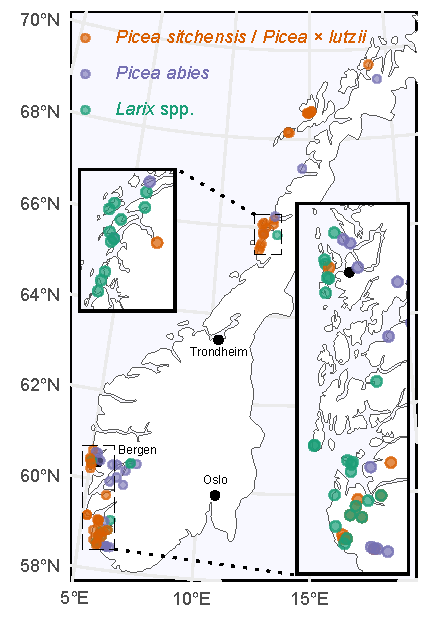
\includegraphics[width=1\linewidth]{figures/sites-map} \caption{Locations of the 82 plantation stands in the sample.}\label{fig:sites-map}
\end{figure}

Within a 2x2 km plot centered on the stand of interest, we mapped all conspecific stands (except in the 2016 field campaign).
Within the central 500x500~m of that plot, we mapped wildlings and ecosystems.
We used GPS to register the point-positions of all wildlings over 30 cm in height, recording a single position for groups of wildlings occurring with less than 5~m between them.
A few exceptionally dense groups of wildlings were mapped by registering polygons instead of points and estimating the number of individuals by transect counts.
Concurrently, we registered polygons for all terrestrial and wetland ecosystems, following the Nature in Norway classification system (version 2.0 or 2.1, Halvorsen et al., \protect\hyperlink{ref-halvorsenNaturNorgeNiN2015}{2015}, based on the principles summarized in Halvorsen et al., \protect\hyperlink{ref-halvorsenSystematicsEcodiversityEcoSyst2020}{2020}).
This system is the national standard for land cover mapping and provides full spatial coverage (i.e.~any location and any kind of land cover is assignable to an ecosystem).
We mapped ecosystems at a scale of 1:5000, which means that any polygon over 250~m\textsuperscript{2} was registered (Bryn \& Halvorsen, \protect\hyperlink{ref-brynVeilederKartleggingAv2015}{2015}).
Regularly patterned occurrence of more than one ecosystem in polygons smaller than the minimum size were registered as so-called mosaic polygons.

For each of the central stands we measured the height of a representative individual by clinometer.
We also estimated the age of the stand at the time of the field campaign, either by contacting land owners and municipal officials, or by counting growth rings.
Details of all 82 stands are provided in the Appendix (table~\ref{tab:sites-table}).

\hypertarget{seed-dispersal}{%
\subsection{Seed dispersal}\label{seed-dispersal}}

To account for the influence of seed dispersal on wildling abundance, we needed estimates of the spatial distribution of seed rain within the 500x500~m plots.
We considered all conspecific stands within a 1 km radius of the central stand to be potential seed sources, and used two models of seed dispersal to derive different estimates of relative seed rain in space.
Acknowledging the uncertainty involved in estimating seed dispersal, we explored one empirically-parameterized, isotropic model and one mechanistically-derived, anisotropic model.

The first model was a static seed dispersal kernel with parameter estimates generalized from multiple data sets.
Specifically, we selected from Bullock et al.~(\protect\hyperlink{ref-bullockSynthesisEmpiricalPlant2017}{2017}) the kernel that performed best for wind-adapted seeds from 5-15~m tall trees (an Exponential Power function).
Seventy-two of the 82 stands in our data set matched this height range better than a taller range with a different empirical kernel.

The second model was an anisotropic implementation of the Wald Analytical Long-distance Dispersal model (WALD, Katul et al., \protect\hyperlink{ref-katulMechanisticAnalyticalModels2005}{2005}), following Skarpaas \& Shea (\protect\hyperlink{ref-skarpaasDispersalPatternsDispersal2007}{2007}).
We parameterized the model with: site- and season-specific wind vectors retrieved from meteorological data sets, wind turbulence estimated from local ecosystem composition, seed release height based on stand height, and species-specific seed terminal velocities from literature.

We transformed field-mapped polygons of potential seed sources into hexagonally gridded point sources, with a density of 0.1~m\textsuperscript{-2} for the first model and 0.01~m\textsuperscript{-2} for the second model (to reduce computation time).
Then we applied our two dispersal models to estimate the distribution of relative seed rain from all point sources in a grid of 10~m cells.
We chose this cell size to be similar to the smallest allowed ecosystem polygon.

A full description of our implementation of the WALD model and additional details about seed source polygons are given in the \protect\hyperlink{appendix}{Appendix}.

\hypertarget{establishment-likelihood}{%
\subsection{Establishment likelihood}\label{establishment-likelihood}}

For our analysis of establishment likelihood, wildling occurrences and ecosystems were rasterized to the same 10~m grid as the seed dispersal models (fig.~\ref{fig:site-example}).
Rather than assigning a single ecosystem to each grid cell, we assigned ecosystems in proportion to their areal coverage of the cell (i.e.~each ecosystem was rendered as a separate raster variable with a {[}0,1{]} range).
This allowed us to capture ecotones in the model and avoid overreliance on the spatial precision of ecosystem boundaries.
Area covered by mosaic polygons was divided evenly among the constituent ecosystem types.
We excluded the ``tree plantation'' ecosystem from our analyses because some of the field campaigns did not register wildlings occurring there.
Grid cells comprised mostly of ``tree plantation'' (\textgreater~0.5) were dropped.
The resulting data set was used to calculate wildling densities (abundance/area) and to model relative establishment likelihoods.
For the density calculation, wildling abundance was tallied in proportion to the ecosystem composition of its grid cell.
For example, a cell occupied by three wildlings and half-covered by a given ecosystem would tally 1.5 wildlings for that ecosystem.

\begin{figure}
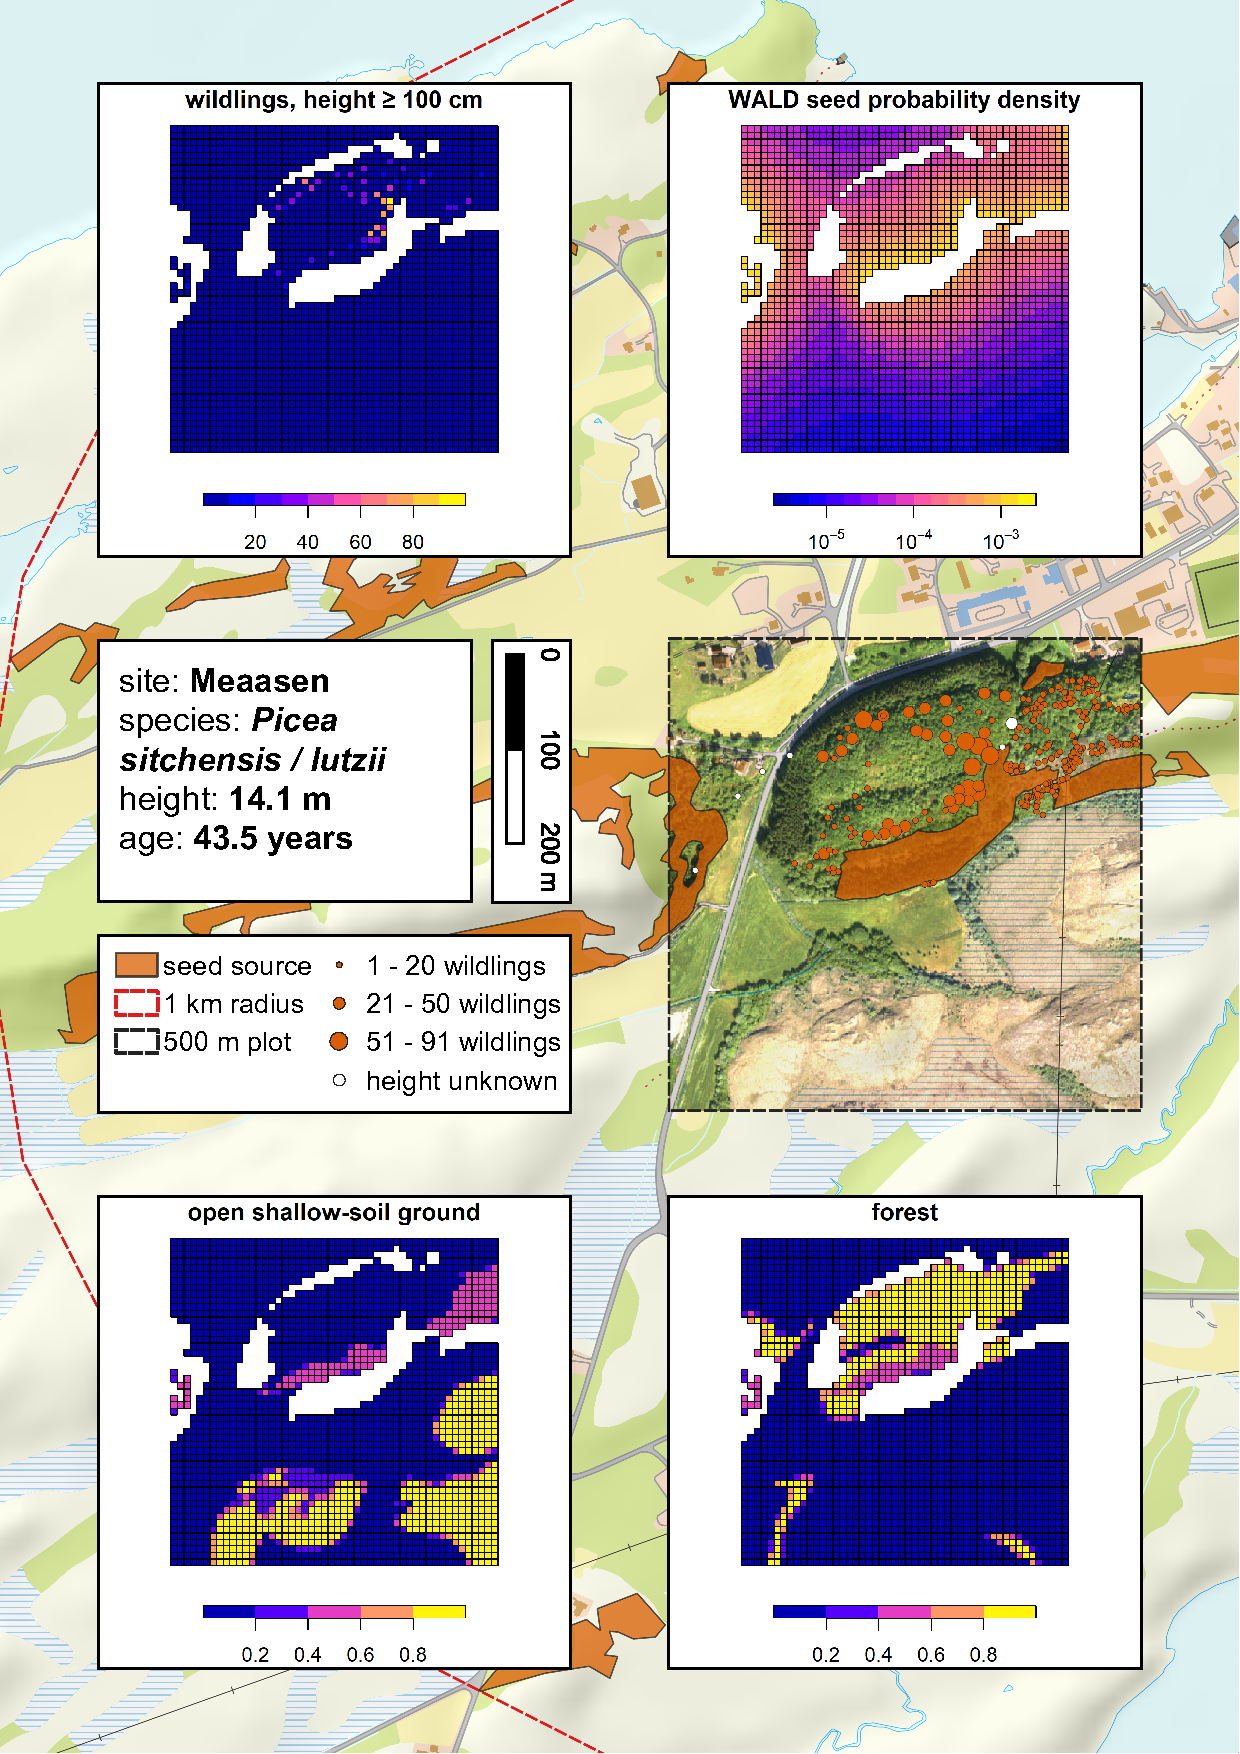
\includegraphics[width=0.9\linewidth]{figures/site-example/site-example} \caption{An illustration of one of the 82 plantations: Meaasen. The background map shows the surroundings of the plantation, and the 500x500 m plot is overlaid with an aerial photograph. The middle row of panels shows the data as registered in the field (but without ecosystem type polygons). The top and bottom rows of panels show selected variables for the 500x500 m plot, as used in the regression model (with a spatial grain of 10 m). Grid cells without data are either seed sources (corresponding to the polygons shown) or "tree plantations" of other species (such as one along the road).}\label{fig:site-example}
\end{figure}

We used a directed acyclic graph (DAG) to diagram causal relationships among the factors we expected to influence wildling abundance per cell (fig.~\ref{fig:DAG}).
In the DAG, the unmeasured, proximate causes of wildling abundance --- total seed rain over the lifetime of the stand and establishment likelihood --- are descendants of variables that we could observe or model.
We included an effect of elevation from the stand on seed rain because neither of our models of seed dispersal account for uneven terrain.

\begin{figure}
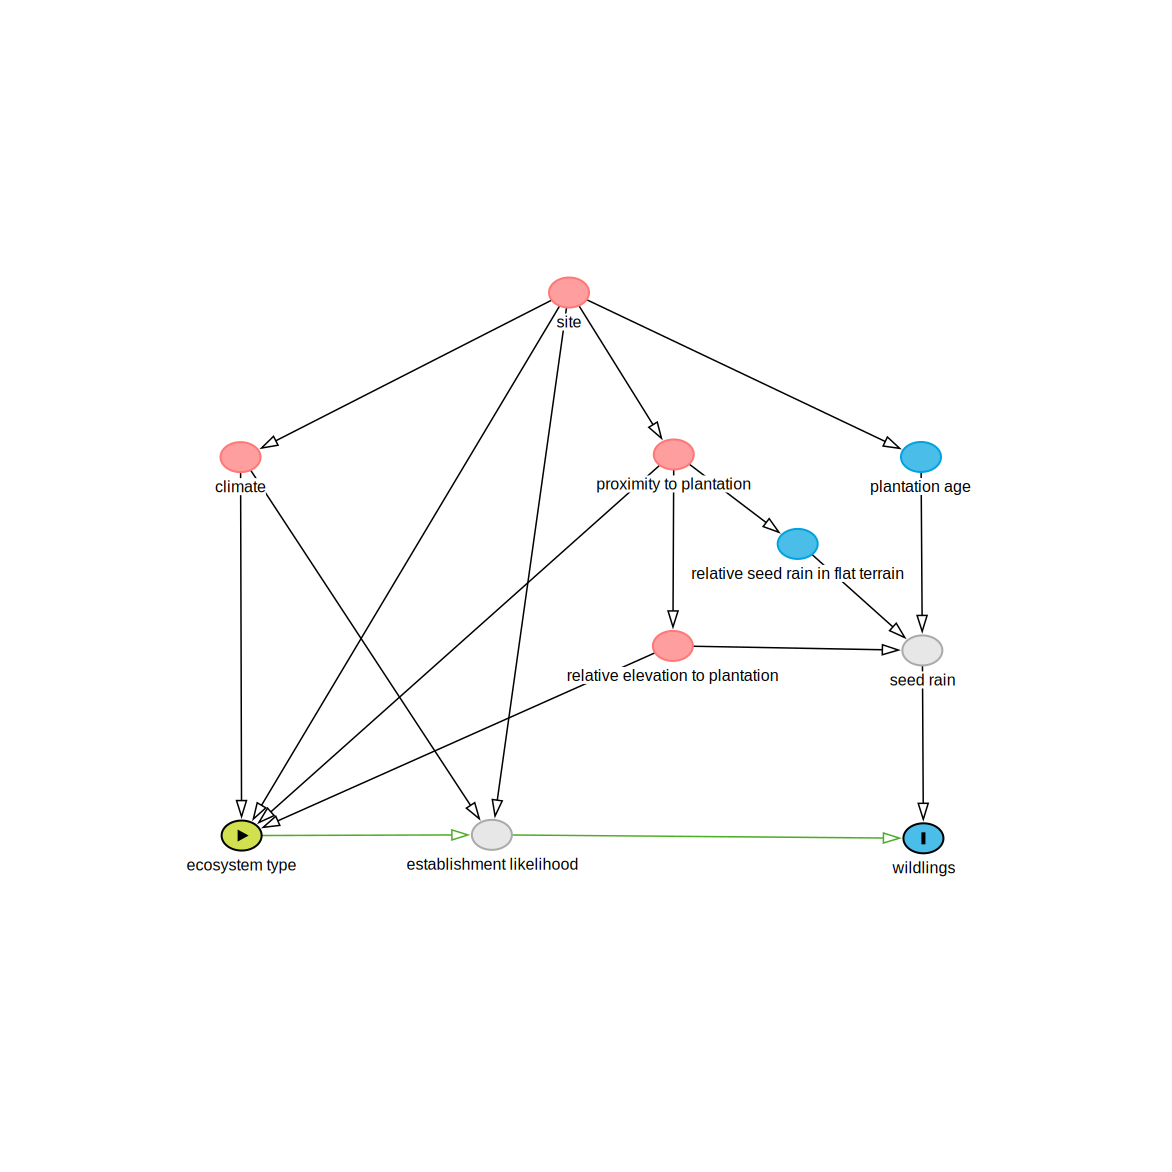
\includegraphics[width=0.9\linewidth]{/home/julien/Documents/dissertation/chapter3/conifer-plantation-spread/ms/figures/dagitty-model} \caption{A directed acyclic graph showing the causal relationships motivating our statistical model of ecosystems' effects on wildling abundance. Red variables causally affect both the ecosystem type and wildling abundance, blue variables causally affect only wildling abundance, and grey variables are unobserved. Green arrows show the causal pathway of interest.}\label{fig:DAG}
\end{figure}

For all species, wildling abundance showed a high frequency of zeros that was underestimated by the best fitting negative binomial distribution.
Accordingly, we applied zero-inflated generalized linear models, fitted with the glmmTMB package (version 1.0, Brooks et al., \protect\hyperlink{ref-brooksGlmmTMBBalancesSpeed2017}{2017}) in R (version 3.6, R Core Team, \protect\hyperlink{ref-rcoreteamLanguageEnvironmentStatistical2020}{2020}).
These zero-inflated models regard zeros as the mixed product of a binomial process as well as a (conditional) count process that can take different error distributions (Zuur et al., \protect\hyperlink{ref-zuurMixedEffectsModels2009}{2009}).
Preliminary models fitted with a negative binomial error distribution in the count process (ZINB) sometimes showed residual underdispersion, so we switched to a generalized Poisson error distribution (ZIGP), which can accommodate both over- and underdispersion (Brooks et al., \protect\hyperlink{ref-brooksStatisticalModelingPatterns2019}{2019}).

We modeled the binomial process as dependent on stand age and site, with site as a random variable.
We expected that younger stands would exhibit more wildling-free cells than predicted under a constant establishment rate from age zero, because of their infertile juvenile period.
We also expected the frequency of zeros to vary with site, because our field work documented that some land owners had occasionally made efforts to remove wildlings.
Excess zeros that arose in these ways would therefore not bias our estimates of establishment likelihood (Blasco-Moreno et al., \protect\hyperlink{ref-blasco-morenoWhatDoesZero2019}{2019}).

To estimate the causal influence of ecosystems on wildling abundance in accordance with the DAG (McElreath, \protect\hyperlink{ref-mcelreathHauntedDAGCausal2020}{2020}; Textor et al., \protect\hyperlink{ref-textorRobustCausalInference2016}{2016}), we modeled the count process as dependent on ecosystem, site, climate, elevation from the stand, and relative seed rain.
We also included stand age in the count process model because it reduced the unexplained variance associated with the random effect of site, and because we could interpret its coefficient as an (unconfounded) total effect on wildling abundance (Westreich \& Greenland, \protect\hyperlink{ref-westreichTableFallacyPresenting2013}{2013}).
Climate was represented as mean annual temperature (Bio1) and precipitation of the coldest quarter (Bio19), at 30~arcsecond resolution, from CHELSA data (Karger et al., \protect\hyperlink{ref-kargerClimatologiesHighResolution2017}{2017}).
We chose these variables because they showed the strongest correlations with Norwegian vegetation zones and sections, respectively (Bakkestuen et al., \protect\hyperlink{ref-bakkestuenSteplessModelsRegional2008}{2008}).
For lodgepole pine we used only Bio19 because the two variables were highly correlated (\(\rho\) = 0.98).
Elevation from the stand was taken with respect to the highest point of the central stand, from digital elevation models at 1 or 10~m resolution (Norwegian Mapping Authority).
Relative seed rain directly represents relative exposure in the count process, so we entered the natural log of this variable as an offset term (coefficient fixed at 1; Zuur et al., \protect\hyperlink{ref-zuurMixedEffectsModels2009}{2009}).
We expect, for example, that a doubling in seed rain would result in a doubling in wildling abundance, all else being equal.

To summarize, for each species we modeled:

\begin{equation}
\begin{aligned}
wildlings_{ijk} &\sim ZIGP(\pi_{i}, \mu_{ijk}, \phi) \\
logit(\pi_{i}) &= StandAge_{i} + Site_{i} \\
log(\mu_{ijk}) &= \sum\limits_{k=1}^K EcosystemType_{ijk} + Site_{i} + Bio1_{i} + Bio19_{i} + \\
&RelativeElevation_{ij} + StandAge_{i} + \\
&offset(log(RelativeSeedRain_{ij})) \\
Site_{i} &\sim Normal(0, \sigma^2) \\
\end{aligned}
\end{equation}

where \(\pi\) is the probability of a zero from the binomial process, while \(\mu\) and \(\phi\) are the mean and dispersion of the generalized Poisson distribution, respectively (Brooks et al., \protect\hyperlink{ref-brooksStatisticalModelingPatterns2019}{2019}).
Subscripts \(i\), \(j\), and \(k\) index sites, cells, and ecosystems.

For each species, ecosystems where wildlings were totally absent were dropped as predictors (to avoid model convergence issues stemming from complete separation), along with the cells that were comprised mostly (\textgreater~0.5) of one of these ecosystems.
The values of Bio1, Bio19, elevation from the stand, and stand age were standardized, and the natural log of relative seed rain was centered.
We fitted three parallel models for each species: (1) with relative seed rain derived from the empirical dispersal kernel, (2) with relative seed rain derived from the WALD dispersal model, and (3) without relative seed rain.
From these three we selected that with the best AIC.
Two models (larches without seed rain and lodgepole pine with empirical dispersal kernel) did not converge and were excluded from selection.
To catch problems with our model specification, we looked for deviation from uniformity in quantile-scaled, simulated residuals, using the DHARMa package (version 0.2.7, Hartig, \protect\hyperlink{ref-hartigDHARMaResidualDiagnostics2020}{2020}).
We also ran DHARMa's tests for residual over/underdispersion and zero-inflation.
Relative establishment likelihoods among ecosystems were calculated as predictions from the conditional count part of the model (holding covariates at their mean values), and scaled by the value for ``forests'' (which were common in the sample).

To test whether higher-level characteristics of ecosystems can be used to generalize patterns of susceptibility, we aggregated ecosystems by their category (terrestrial or wetland) and structuring process (none, environmental stress, regulating disturbance, destabilizing disturbance, moderate anthropogenic disturbance, or strong anthropogenic disturbance), as defined in the Nature in Norway system (Appendix, table~\ref{tab:types-table}).
We then refitted our four selected models with these eight strata replacing ecosystems, and obtained estimates of relative establishment likelihood for each category and structuring process.

\hypertarget{results}{%
\section{Results}\label{results}}

Wildling densities across ecosystems ranged 0-211/ha for Sitka/Lutz spruce (unstratified mean: 28), 0-49/ha for Norway spruce (unstratified mean: 6), 0-1045/ha for larches (unstratified mean: 13), and 0-219/ha for lodgepole pine (unstratified mean: 34).
Relative establishment likelihoods differed considerably from relative wildling densities, except in larches (table~\ref{tab:estimate-correlation-table}).
For instance, our model estimated that Sitka/Lutz spruce is three times more likely to establish in ``boreal heath'' than in ``artificial substrate'', despite wildling density being three times lower in ``boreal heath'' (fig.~\ref{fig:establishment}).
The magnitude of variation in relative establishment likelihoods generally matched or exceeded the magnitude of variation in corresponding wildling densities (Appendix table~\ref{tab:dispersion-table}).

\begin{table}

\caption{\label{tab:estimate-correlation-table}Correlations between wildling densities and relative establishment likelihoods across ecosystem types, for each species group.}
\centering
\begin{tabular}[t]{>{}lrr}
\toprule
species group & Pearson & Spearman\\
\midrule
\em{Picea sitchensis / lutzii} & 0.23 & 0.55\\
\em{Picea abies} & 0.22 & 0.73\\
\em{Larix spp.} & 1.00 & 0.89\\
\em{Pinus contorta} & 0.07 & 0.38\\
\bottomrule
\end{tabular}
\end{table}

\newpage
\begin{landscape}

\begin{figure}
\centering
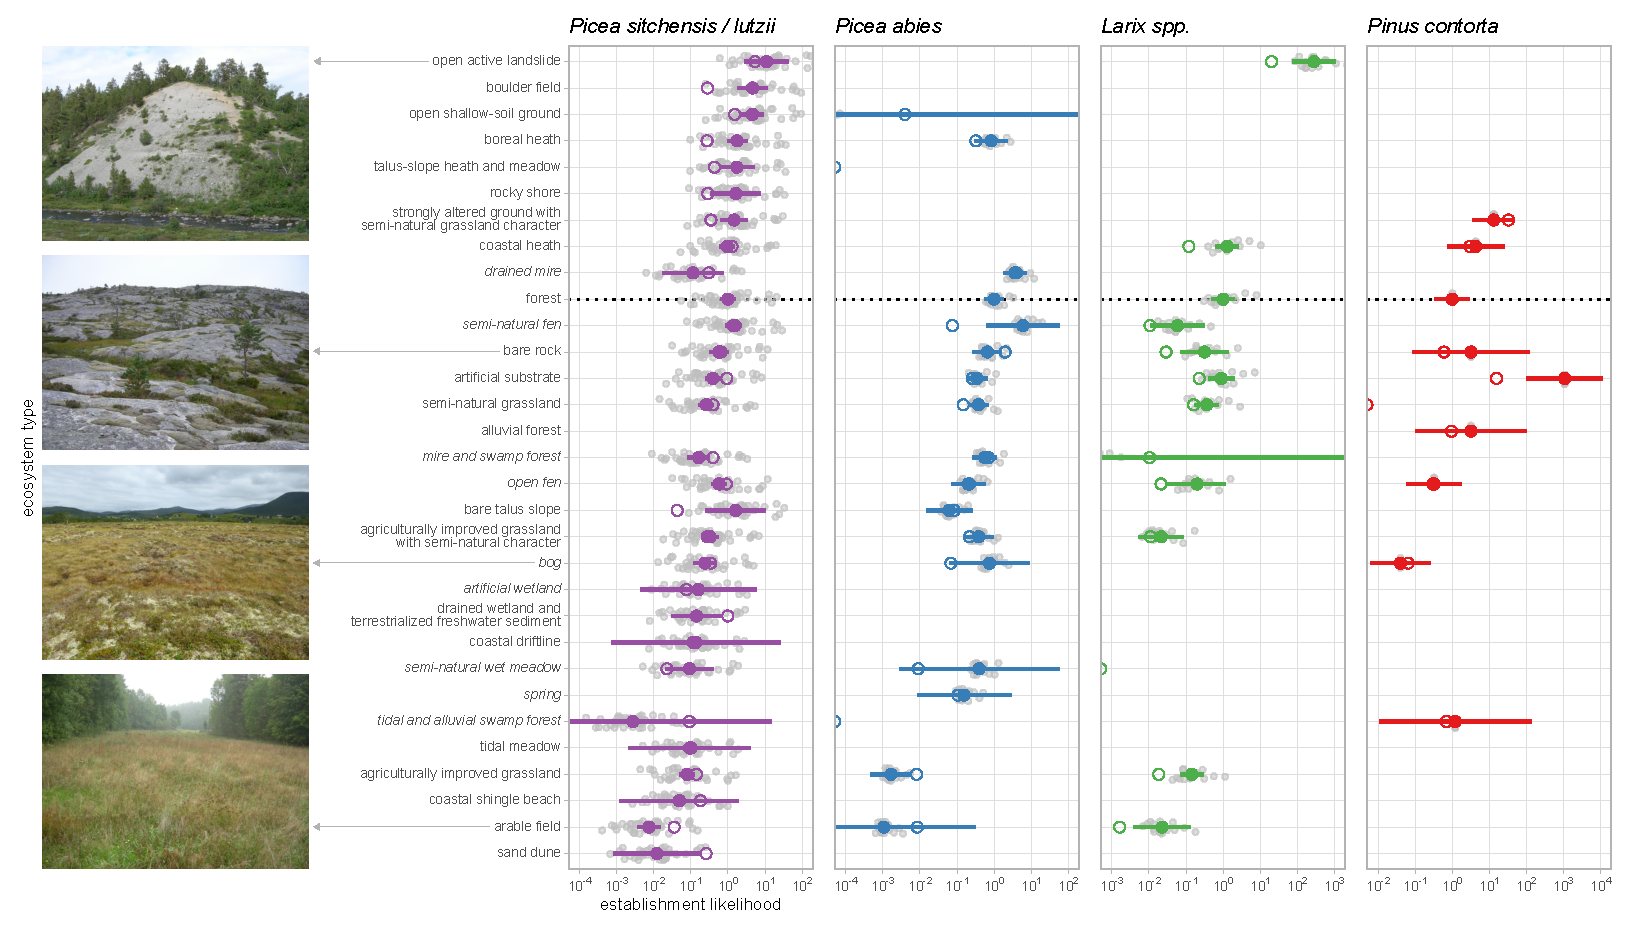
\includegraphics{/home/julien/Documents/dissertation/chapter3/conifer-plantation-spread/ms/figures/establishment/establishment.pdf}
\caption{\label{fig:establishment}Relative densities (unfilled points) and relative establishment likelihoods (filled points) of four alien conifer species groups across ecosystem types, using `forest' as the reference type. Zero density is plotted at the lower limit of the x-axis. Relative establishment likelihoods are shown with 95 \% confidence intervals. Grey points depict relative establishment likelihoods for individual sites in our data set. The order of ecosystem types along the y-axis is determined by a confidence-weighted mean of their percentile-ranked establishment likelihoods within species, such that types with consistently high establishment likelihood across species are at the top. Photos licensed CC BY 4.0 Rune Halvorsen.}
\end{figure}

\end{landscape}
\newpage

For all species, models using relative seed rain estimates from the WALD dispersal model predicted wildling abundance best (Appendix, table~\ref{tab:model-comparison-table}).
Omitting seed rain altogether produced better model fits than using estimates from the empirical dispersal kernel.
Site had a strong influence on wildling abundance for Sitka/Lutz spruce and lodgepole pine, such that site variation swamped much of the variation between ecosystems, for these species.
The direct effects of climate on establishment likelihood varied by species and was strongest for larches (Appendix, tables~\ref{tab:Ps}-\ref{tab:Pc}).
The direct effects of elevation from the stand on wildling abundance (through seed rain) were comparatively modest and acted in different directions for different species.
Stand age did not significantly affect wildling abundance in any species, except that older stands of Sitka/Lutz spruce had fewer wildling-free cells (structural zeros) than younger stands.

Among ecosystems with at least one wildling, estimated establishment likelihoods varied by 3--5 orders of magnitude for the different species.
Patterns of relative establishment likelihood were modestly similar between species, with positive rank correlations in four of six species pairs (table~\ref{tab:species-correlation-table}).
``Arable fields'' showed some of the lowest establishment likelihoods of any ecosystem for all species where it appeared.
Meanwhile, ecosystems with high establishment likelihoods tended to be rarer types (e.g.~``open active landslides'') but also included ``boreal heath'' and ``coastal heath''.

\begin{table}

\caption{\label{tab:species-correlation-table}Spearman correlations of relative establishment likelihoods in ecosystem types, between pairs of species groups.}
\centering
\begin{tabular}[t]{>{}llll}
\toprule
\em{ } & \em{Picea abies} & \em{Larix spp.} & \em{Pinus contorta}\\
\midrule
\em{Picea sitchensis / lutzii} & 0.37 & 0.5 & 0.12\\
\em{Picea abies} &  & 0.18 & -0.1\\
\em{Larix spp.} &  &  & -0.1\\
\bottomrule
\end{tabular}
\end{table}

Variation in establishment likelihoods shrank when ecosystems were aggregated by category or structuring process, to 0--3 orders of magnitude (fig.~\ref{fig:establishment-hypotheses}).
None of the species showed large differences in establishment likelihood between terrestrial and wetland ecosystems.
At most, larches and lodgepole pine were three times less likely to establish in wetlands.
Ecosystems structured by destabilizing disturbance tended to show higher establishment likelihoods than those structured by environmental stress and those without disturbance structuring.
However, the association between structuring process and establishment likelihood was heterogeneous across species.

\newpage
\begin{landscape}

\begin{figure}
\centering
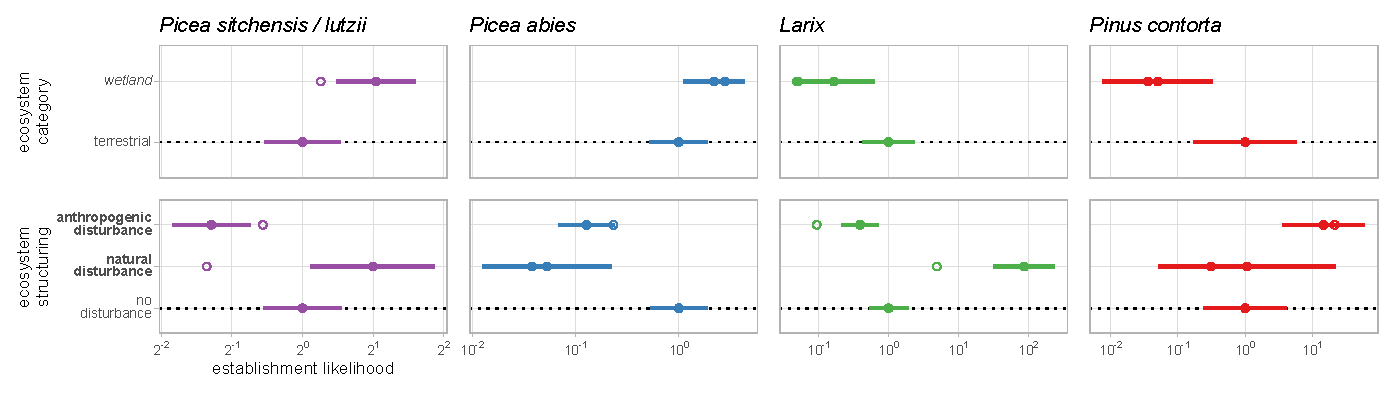
\includegraphics{/home/julien/Documents/dissertation/chapter3/conifer-plantation-spread/ms/figures/establishment-hypotheses.pdf}
\caption{\label{fig:establishment-hypotheses}Relative densities (unfilled points) and relative establishment likelihoods (filled points) of four alien conifer species groups among categories of ecosystem types (top) or structuring processes in ecosystem types (bottom). Relative establishment likelihoods are shown with 95 \% confidence intervals. The horizontal dotted lines indicate the reference strata.}
\end{figure}

\end{landscape}
\newpage

\hypertarget{discussion}{%
\section{Discussion}\label{discussion}}

\hypertarget{how-does-wildling-abundance-relate-to-ecosystem-susceptibility}{%
\subsection{How does wildling abundance relate to ecosystem susceptibility?}\label{how-does-wildling-abundance-relate-to-ecosystem-susceptibility}}

Confounders of the relationship between ecosystem type and wildling abundance caused wildling density to mischaracterize differences in establishment likelihood between ecosystems.
For example, the density of Sitka/Lutz spruce wildlings was about equal in ``bare talus slopes'' and ``arable fields'', but we estimate that establishment likelihood is actually about 1000 times higher in the former.
The nonzero effects of hypothesized confounders (like seed rain, climate, and site) imply that our modeled estimates of establishment likelihood are less biased measures of ecosystem susceptibility.
Furthermore, variation in establishment likelihood was no smaller than variation in wildling densities, as might have been the case if confounding variables had amplified differences in ecosystem establishment.

Because wildling abundance is the product of seed rain and establishment likelihood, we needed to estimate seed rain independently of our wildling data to model establishment likelihood properly.
By including relative seed rain as an offset in the model, we ensured that seed rain and establishment likelihood were not conflated, at the cost of assuming that our relative seed rain estimates were accurate.
Exploring the alternative, we found that if we included relative seed rain as a covariate rather than an offset that its coefficient was estimated near one, and that estimated relative establishment likelihoods remained mostly unchanged (Appendix, fig.~\ref{fig:establishment-sensitivity}).
This result is consistent with the assumption that our WALD-derived estimates of relative seed rain capture true differences in seed rain.
Although survivorship bias in our data prevents rigorous comparison of seed dispersal models, the superior fits of models with WALD-derived seed rain offsets compared to models with empirically-derived seed rain offsets also supports the WALD model estimates.
Lastly, the mechanistic nature of the WALD model makes us more confident in its estimates across species and sites than we would be in a purely phenomenological model (Bullock et al., \protect\hyperlink{ref-bullockAllDispersalFunctions2018}{2018}).
Nevertheless, that seed rain was was modeled and not measured is a limitation of our method, and it makes the establishment likelihoods we estimate less certain.
For example, changes in the distribution of seed rain as a stand matures were not accounted for, nor was secondary seed dispersal from the few reproductive wildlings we observed.

The inconsistent effects of elevation from the stand on wildling abundance suggests that terrain does not affect seed dispersal much or that vertical distance alone misses its effect.
In any case, there is no rule of thumb for management that wildlings tend to move up or down slopes.
Similarly, the weak and inconsistent effects of stand age on wildling abundance suggests that wildlings accumulate sporadically, and that other site characteristics tend to outweigh the effect of age.

Our models do not estimate climate's total causal effect on wildling abundance, because they set aside its influence on ecosystems (Westreich \& Greenland, \protect\hyperlink{ref-westreichTableFallacyPresenting2013}{2013}).
Therefore, we interpret the estimated climatic effects with respect to physiological constraints within a given ecosystem.
The negligible effect of precipitation and weakly positive effect of mean annual temperature on Sitka/Lutz spruce wildling abundance is consistent with Sitka spruce's wide climatic tolerance relative to climatic variation in Norway and its oceanic affinity (Peterson et al., \protect\hyperlink{ref-petersonEcologyManagementSitka1997}{1997}).
For Norway spruce, our results support a previous finding that seedling recruitment increases towards the wetter end of Norwegian climate (Tingstad et al., \protect\hyperlink{ref-tingstadTemperaturePrecipitationBiotic2015}{2015}), although most of our sites circumscribed a narrow part of that range.
Warm and wet conditions seem to suppress larch establishment in Norway, which may be taken into consideration when managing these plantations.

A curious feature of our results that needs more research is the large amount of unexplained variation in Sitka/Lutz spruce and lodgepole pine wildling abundance between sites.
This means that our ability to predict the spread of these species at a specific site, relative to other sites, is limited (even if the site's ecosystem composition is known).
Nevertheless, ecosystem comparisons can and should guide management.
Bianchi et al.~(\protect\hyperlink{ref-bianchiMethodsPredictingSitka2019}{2019}) struggled to predict regeneration density within Sitka spruce plantations from stand density (among other predictors), which suggests that the unexplained site-level variation in our models was not caused by our assumption of constant seed source density.
Alternative explanations could include: (1) property owners removing wildlings, (2) disturbance legacies not captured in the delineation of ecosystem types (especially in grazing pressure; Miller et al., \protect\hyperlink{ref-millerHowDisturbanceHistory2021}{2021}), or (3) differing demographic characteristics among plantations (especially in cone production; Taylor et al., \protect\hyperlink{ref-taylorDriversPlantInvasion2016}{2016}), potentially as a result of provenance.
Ecological differences between Lutz and Sitka spruce might also explain some of the site variation in that case.

\hypertarget{which-ecosystems-are-susceptible}{%
\subsection{Which ecosystems are susceptible?}\label{which-ecosystems-are-susceptible}}

In a large database of vegetation plots across Europe, Chytrý et al.(\protect\hyperlink{ref-chytryHabitatInvasionsAlien2008}{2008}) found that alien plants as a group are consistently found at low rates in mires and heaths, and high rates in arable, man-made, and coastal ecosystems.
The conifer species we examined do not conform closely to these broader trends in ecosystem invasibility, showing relatively high rates of establishment in heaths and very low rates of establishment in arable ecosystems.
To the extent that there are similarities across these four species, they appear to establish more easily in ecosystems infrequently hit by intense disturbances (e.g.~rock fall in ``bare talus slope'') than in ecosystems frequently experiencing less intense disturbances (e.g.~flooding in ``semi-natural wet meadow'').

Of the species in this study, lodgepole pine's establishment is best studied, and our results are consistent with this literature.
``Bare rock'' harbors very few competitors and showed highest lodgepole pine establishment of all ecosystems (Despain, \protect\hyperlink{ref-despainDispersalEcologyLodgepole2001}{2001}), and ecosystems with canopy cover generally showed low establishment (Langdon et al., \protect\hyperlink{ref-langdonPinusContortaInvasion2010}{2010}; Taylor et al., \protect\hyperlink{ref-taylorDriversPlantInvasion2016}{2016}).
It is difficult to evaluate our ecosystem susceptibility results against the recruitment patterns that have been described for the three other species.
For instance, Sitka spruce grows poorly under moisture stress and tolerates flooding well (Peterson et al., \protect\hyperlink{ref-petersonEcologyManagementSitka1997}{1997}), which might account for why it was equally likely to establish in wetland and terrestrial ecosystems.
Yet it also established well in ``open shallow-soil ground'', despite this ecosystem's characteristically dry soil.
This illustrates the trouble with deriving predictions from generalized statements about species autecology.
Furthermore, ecosystems that would seem inhospitable based on their overall characteristics may actually contain many localized opportunities for establishment, because seedling mortality is strongly regulated by microsites (Macek et al., \protect\hyperlink{ref-macekLifeDeathPicea2017}{2017}).
From this perspective, our estimates of establishment likelihood measure the density of suitable microsites in a given ecosystem.

The breadth in establishment likelihood suggests that differences between ecosystems deserve careful consideration when managing wildling spread.
This knowledge may be applied in at least two ways.
First, as a preventative measure, we recommend siting new stands where surrounded by high proportions of ecosystems with low establishment likelihood.
In particular, ``arable fields'' repress wildling establishment for all species and are common near existing stands, so picking sites hemmed in by this kind of agricultural land should be both effective and feasible.
This would probably reduce the rate of wildling establishment by orders of magnitude, even if long distance dispersal might preclude complete containment (Albert et al., \protect\hyperlink{ref-albertLanduseChangeSubalpine2008}{2008}).
In some cases it may also be desirable to transform ecosystems adjacent to existing stands to prevent (further) spread, for example by intensifying mowing regimes to promote the appearance of ``agriculturally improved grassland''.
Second, as a reactive measure, we recommend allocating resources for monitoring and control in proportion to relative ecosystem susceptibility.
Prioritizing ecosystems that are highly susceptible and also rare (e.g.~``open active landslide'') is especially likely to be cost-efficient.

The establishment patterns we quantify probably hold, more or less, beyond Norway (Chytrý, Maskell, et al., \protect\hyperlink{ref-chytryHabitatInvasionsAlien2008}{2008}).
From a manager's perspective, we expect that the ecosystems we report may translate well to equivalent types in similar classification systems, because the Nature in Norway classification is rule-based and aims for observer neutrality.
At the same time, we urge caution in extending our establishment estimates to ecosystems that are only broadly similar, because we found that similar types frequently showed markedly different susceptibility (e.g.~Norway spruce in ``agriculturally improved grassland with semi-natural character'' vs.~``agriculturally improved grassland'').

An observational study like ours informs management of long-lived, naturalized species more directly than experimental studies, because longer time frames are examined.
It measures long-term survival --- often the quantity of interest --- under a wide range of natural conditions experienced by the wildlings.
In contrast, seeding experiments generally observe only the youngest life stages, and the factors controlling individual success differ at later life stages (Dovčiak et al., \protect\hyperlink{ref-dovciakSeedRainEnvironmental2008}{2008}).
For example, Sitka spruce appears more likely to germinate in disturbed soil (Vikane et al., \protect\hyperlink{ref-vikaneInvasionCallunaHeath2013}{2013}), but less likely to survive there (Peterson et al., \protect\hyperlink{ref-petersonEcologyManagementSitka1997}{1997}).
On the other hand, experiments might be more useful when observed wildling spread is not representative of patterns in the wider landscape (e.g.~for species expanding from a single, recent introduction).

\hypertarget{what-do-susceptible-ecosystems-have-in-common}{%
\subsection{What do susceptible ecosystems have in common?}\label{what-do-susceptible-ecosystems-have-in-common}}

The overarching characteristics that we used to aggregate ecosystems did not generalize differences in susceptibility well, especially not across species, so these classifications have limited utility for management.
Note that different sets of ecosystems comprised the strata for each species, depending on their presence in the data, and these differences in ecosystem composition help explain why the patterns of aggregated establishment likelihood varied between species.
This constraint hinders species comparisons but underlines our main takeaway from these results --- that the susceptibility of an individual ecosystem frequently diverges from those it is classified with.

Within species, we urge careful interpretation of the comparisons among ecosystem categories and structuring processes.
Many areas where conifer establishment is nearly impossible, like paved surfaces and annually plowed fields, count as terrestrial and strongly anthropogenically disturbed, which lowers the relative establishment likelihood of these two strata.
Our results do not imply, for example, that a strong anthropogenic disturbance event will decrease establishment likelihood of Sitka/Lutz spruce relative to an ecosystem's prior state Indeed, Vikane et al.~(\protect\hyperlink{ref-vikaneInvasionCallunaHeath2013}{2013}) show, for example, that burning in coastal heath increases Sitka spruce establishment.
Rather, we find that ecosystems structured by strong anthropogenic disturbance, on the whole, are less susceptible to Sitka/Lutz spruce wildlings than other ecosystems.

\hypertarget{conclusions}{%
\section{Conclusions}\label{conclusions}}

One of the main novelties of this study is that we inferred susceptibility/invasibility using mechanistically reconstructed, spatial estimates of seed rain.
Scientists studying invasibility at national and continental scales have already recognized the importance of normalizing observed levels of invasion by a spatially explicit estimate of exposure (i.e.~propagule pressure; Chytrý, Jarošík, et al., \protect\hyperlink{ref-chytrySeparatingHabitatInvasibility2008}{2008}).
However, many studies quantifying ecosystem invasibility have not been able to adjust for propagule pressure, typically because it is impossible to reconstruct the underlying dispersal history (Catford et al., \protect\hyperlink{ref-catfordQuantifyingLevelsBiological2012}{2012}).
We found that accounting for seed rain and other confounders of the relationship between ecosystems and wildling abundance reshuffles estimates of ecosystem invasibility considerably.

Wildling spread from plantations is a growing problem (Richardson \& Rejmánek, \protect\hyperlink{ref-richardsonConifersInvasiveAliens2004}{2004}) and will probably worsen with recent pushes to increase tree planting worldwide (Brundu et al., \protect\hyperlink{ref-brunduGlobalGuidelinesSustainable2020}{2020}).
Meanwhile, remotely sensed and surveyed data are increasing the availability of detailed and accurate maps of ecosystems across large areas, which presents opportunities to manage wildling spread more efficiently.
Specifically, differences in ecosystem susceptibility may be leveraged to
reduce the rate of wildling establishment through deliberate site selection for new stands or targeted interventions around existing stands.
However, managers should not judge ecosystem susceptibility based on wildling density alone, nor on generalizations across ecosystems.

\hypertarget{authors-contributions}{%
\section{Authors' contributions}\label{authors-contributions}}

JV, SLO, and OSk conceived the ideas and designed methodology; SLO, LA, MOK, AO, JS, OSt, and ØS collected the data; JV analyzed the data and led the writing. All authors contributed to drafts and gave approval for publication.

\hypertarget{acknowledgements}{%
\section{Acknowledgements}\label{acknowledgements}}

We thank Honorata Gajda, Knut Børge Strøm, Heidi Elin Myklebost, Jon Hagelin, Vigdis Frivoll, Sina Thu Randulff, Roy Mangersnes, Bjarne Homnes Oddane, Rune Søyland, Solbjørg Engen Torvik, Toralf Tysse, Craig Jackson, Miene-Marie Gastinger, Ola Westby Aamodt, and Anders Ringstad for their help in collecting and/or collating the field data. Field work was financed by the Norwegian Environment Agency (contracts \#15040036, \#17070025, \#19087470, \#19087471\ldots).

\newpage

\hypertarget{appendix}{%
\section{Appendix}\label{appendix}}

The WALD model (Katul et al., \protect\hyperlink{ref-katulMechanisticAnalyticalModels2005}{2005}) takes the form of an inverse Gaussian distribution whose mean (\(\mu\)) and shape (\(\lambda\)) parameters are calculated from physical characteristics of the dispersal system:

\begin{equation}
\mu  = \frac{HU}{F}
\end{equation}
\begin{equation}
\lambda = \left(\frac{H}{\sigma}\right)^2
\end{equation}

where \(H\) is the seed release height, \(U\) is the mean horizontal wind velocity between \(H\) and the ground, \(F\) is the terminal velocity of the seed, and \(\sigma\) is a wind turbulence parameter.
We set \(H\) to the height of the central stand, estimated \(U\) from a computed vertical wind profile, obtained \(F\) from literature, and calculated \(\sigma\) from an equation for turbulent flow as a function of vegetation height (eq. A4 in Skarpaas \& Shea, \protect\hyperlink{ref-skarpaasDispersalPatternsDispersal2007}{2007}).
We parameterized separate WALD models for 20º sectors around each seed source, to make seed dispersal anisotropic (directional).
In each sector we estimated mean vegetation height based on the composition of mapped ecosystem types (Appendix, table~\ref{tab:types-table}).
Simultaneously, we randomly sampled 100 wind velocities in the direction of the sector during the species' dispersal season.
The 100 resulting WALD kernels produced the seed probability density in the sector, and individual sectors were weighed by the frequency of corresponding wind directions (again, during the species' dispersal season).
The wind data were obtained either from the nearest weather station (MET Norway), a 2.5 km resolution interpolated hindcast covering southern Norway (Haakenstad \& Haugen, \protect\hyperlink{ref-haakenstad15yearHighResolution2017}{2017}), or a 10 km resolution hindcast covering all of Norway (Haakenstad et al., \protect\hyperlink{ref-haakenstadNORA10EIRevisedRegional2020}{2020}; Reistad et al., \protect\hyperlink{ref-reistadHighresolutionHindcastWind2011}{2011}). We used weather station data if the station was less than 2.5 or 10 km away (depending on hindcast coverage), or else the highest resolution hindcast.

\newpage

\begin{ThreePartTable}
\begin{TableNotes}
\item \textit{References: } 
\item 1. Harris, A. S. Sitka spruce. in Silvics of North America: 1. Conifers (eds. Burns, R. M. \& Honkala, B. H.) vol. 2 513–529 (U.S. Department of Agriculture, Forest Service, 1990).
\item 2. Sandvik, H. Kunnskapsstatus for spredning og effekter av fremmede bartrær på biologisk mangfold. (2012).
\item 3. Sullivan, J. Larix decidua. Fire Effects Information System, U.S. Department of Agriculture, Forest Service, Rocky Mountain Research Station,  Fire Sciences Laboratory https://www.fs.fed.us/database/feis/plants/tree/lardec/all.html (1994).
\item 4. Sullivan, J. Picea abies. Fire Effects Information System, U.S. Department of Agriculture, Forest Service, Rocky Mountain Research Station,  Fire Sciences Laboratory https://www.fs.fed.us/database/feis/plants/tree/picabi/all.html (1994).
\end{TableNotes}
\begin{longtable}[t]{>{}llll}
\caption{\label{tab:traits-table}Dispersal traits}\\
\toprule
species group & seed terminal velocity & dispersal season & references\\
\midrule
\em{Larix spp.} & 1.0 m/s & Dec - May & 2, 3\\
\em{Picea abies} & 0.58 m/s & Nov - May & 2, 4\\
\em{Pinus contorta} & 0.82 m/s & Sep - Dec & 2\\
\em{Picea sitchensis / lutzii} & 0.94 m/s & Oct - Feb & 1, 2\\
\bottomrule
\insertTableNotes
\end{longtable}
\end{ThreePartTable}

Some of the seed source polygons we registered in the field had distinctive features that we accounted for as follows.
Seed source polygons for which the species of interest only made up a fraction of the stand composition (e.g.~in Olsen et al., \protect\hyperlink{ref-olsenKartleggingAvKortdistansespredning2019}{2019}) were used with their point source density adjusted accordingly.
For example, a stand identified as composed of Sitka spruce and Norway spruce was assigned a seed source point density half that of a Sitka spruce monoculture.
Likewise, `mixed forest' stands (e.g.~in Appelgren, \protect\hyperlink{ref-appelgrenKartleggingAvKortdistansespredning2018}{2018}) were assigned 0.1 times the seed source point density of a monoculture.\\
Seed source polygons identified as logged (e.g.~in Appelgren, \protect\hyperlink{ref-appelgrenKartleggingAvKortdistansespredning2018}{2018}) were included as seed sources only if we could confirm that they were logged no earlier the decade prior to mapping, using time series of aerial photos.

\begin{landscape}
\begin{longtable}[t]{l>{}llllllll}
\caption{\label{tab:sites-table}\label{tab:sites-table}Plantation stands}\\
\toprule
reference & species group & site & easting & northing & height & age & bio01\textsuperscript{a} & bio19\textsuperscript{b}\\
\midrule
\endfirsthead
\caption[]{\label{tab:sites-table}Plantation stands \textit{(continued)}}\\
\toprule
reference & species group & site & easting & northing & height & age & bio01\textsuperscript{a} & bio19\textsuperscript{b}\\
\midrule
\endhead

\endfoot
\bottomrule
\multicolumn{9}{l}{\rule{0pt}{1em}\textit{Note: }}\\
\multicolumn{9}{l}{\rule{0pt}{1em}Easting and Northing are given for UTM zone 33N. Height is given in meters and age in years.}\\
\multicolumn{9}{l}{\rule{0pt}{1em}\textsuperscript{a} mean annual temperature (°C)}\\
\multicolumn{9}{l}{\rule{0pt}{1em}\textsuperscript{b} precipitation in coldest quarter (cm)}\\
\multicolumn{9}{l}{\rule{0pt}{1em}\textsuperscript{*} interpolated as the mean height of conspecific stands, inversely weighted by difference in age}\\
\multicolumn{9}{l}{\rule{0pt}{1em}\textsuperscript{\dag} interpolated as the mean age of conspecific stands in the same region}\\
\endlastfoot
\cellcolor{gray!6}{Olsen et al. 2016} & \em{\cellcolor{gray!6}{Pinus contorta}} & \cellcolor{gray!6}{Fiskvikrokkdalen} & \cellcolor{gray!6}{292498} & \cellcolor{gray!6}{6843676} & \cellcolor{gray!6}{11} & \cellcolor{gray!6}{58} & \cellcolor{gray!6}{2.36} & \cellcolor{gray!6}{12.8}\\
Olsen et al. 2016 & \em{Pinus contorta} & Gulemyrane & 94625 & 7000110 & 9\textsuperscript{*} & 42 & 7.22 & 48.0\\
\cellcolor{gray!6}{Olsen et al. 2016} & \em{\cellcolor{gray!6}{Pinus contorta}} & \cellcolor{gray!6}{Selvik} & \cellcolor{gray!6}{74593} & \cellcolor{gray!6}{6978018} & \cellcolor{gray!6}{8} & \cellcolor{gray!6}{45} & \cellcolor{gray!6}{7.25} & \cellcolor{gray!6}{40.0}\\
Olsen et al. 2016 & \em{Pinus contorta} & Skarsheia & 78833 & 6979095 & 6 & 45 & 6.60 & 36.7\\
\cellcolor{gray!6}{Olsen et al. 2016} & \em{\cellcolor{gray!6}{Pinus contorta}} & \cellcolor{gray!6}{Sollitangen} & \cellcolor{gray!6}{260896} & \cellcolor{gray!6}{6859024} & \cellcolor{gray!6}{12} & \cellcolor{gray!6}{37} & \cellcolor{gray!6}{2.60} & \cellcolor{gray!6}{6.7}\\
\addlinespace
Olsen et al. 2016 & \em{Pinus contorta} & Tomasmyra & 260694 & 6864426 & 12 & 29 & 2.44 & 6.2\\
\cellcolor{gray!6}{Olsen et al. 2016} & \em{\cellcolor{gray!6}{Picea sitchensis / lutzii}} & \cellcolor{gray!6}{Gryttingdalen-vest} & \cellcolor{gray!6}{503887} & \cellcolor{gray!6}{7613803} & \cellcolor{gray!6}{8} & \cellcolor{gray!6}{52} & \cellcolor{gray!6}{4.56} & \cellcolor{gray!6}{49.0}\\
Olsen et al. 2016 & \em{Picea sitchensis / lutzii} & Gryttingdalen-oest & 504335 & 7613736 & 8 & 52 & 4.50 & 50.5\\
\cellcolor{gray!6}{Olsen et al. 2016} & \em{\cellcolor{gray!6}{Picea sitchensis / lutzii}} & \cellcolor{gray!6}{Holmsnes-nordvest} & \cellcolor{gray!6}{493935} & \cellcolor{gray!6}{7609464} & \cellcolor{gray!6}{11} & \cellcolor{gray!6}{49} & \cellcolor{gray!6}{5.36} & \cellcolor{gray!6}{45.3}\\
Olsen et al. 2016 & \em{Picea sitchensis / lutzii} & Holmsnes-soeroest & 494675 & 7608420 & 11 & 45 & 5.46 & 44.0\\
\addlinespace
\cellcolor{gray!6}{Olsen et al. 2016} & \em{\cellcolor{gray!6}{Picea sitchensis / lutzii}} & \cellcolor{gray!6}{Hov} & \cellcolor{gray!6}{496920} & \cellcolor{gray!6}{7608739} & \cellcolor{gray!6}{11} & \cellcolor{gray!6}{56} & \cellcolor{gray!6}{5.22} & \cellcolor{gray!6}{50.9}\\
Olsen et al. 2016 & \em{Picea sitchensis / lutzii} & Raavollmarka & 499105 & 7608885 & 18 & 59 & 4.80 & 51.1\\
\cellcolor{gray!6}{Appelgren and Torvik 2017} & \em{\cellcolor{gray!6}{Larix spp.}} & \cellcolor{gray!6}{Anisdal} & \cellcolor{gray!6}{-36439} & \cellcolor{gray!6}{6529890} & \cellcolor{gray!6}{22} & \cellcolor{gray!6}{56} & \cellcolor{gray!6}{7.37} & \cellcolor{gray!6}{38.8}\\
Appelgren and Torvik 2017 & \em{Larix spp.} & Haalandsbotn & -37108 & 6532830 & 20 & 57.5 & 7.00 & 38.9\\
\cellcolor{gray!6}{Appelgren and Torvik 2017} & \em{\cellcolor{gray!6}{Larix spp.}} & \cellcolor{gray!6}{Roeynaasen} & \cellcolor{gray!6}{-31279} & \cellcolor{gray!6}{6547997} & \cellcolor{gray!6}{25} & \cellcolor{gray!6}{77.5} & \cellcolor{gray!6}{6.88} & \cellcolor{gray!6}{36.5}\\
\addlinespace
Appelgren and Torvik 2017 & \em{Larix spp.} & Storemo & -107 & 6588189 & 23 & 60 & 7.15 & 33.0\\
\cellcolor{gray!6}{Appelgren and Torvik 2017} & \em{\cellcolor{gray!6}{Larix spp.}} & \cellcolor{gray!6}{Toegjefjellet} & \cellcolor{gray!6}{-22293} & \cellcolor{gray!6}{6546411} & \cellcolor{gray!6}{20} & \cellcolor{gray!6}{60} & \cellcolor{gray!6}{6.69} & \cellcolor{gray!6}{39.6}\\
Appelgren and Torvik 2017 & \em{Larix spp.} & Voren & -26899 & 6554824 & 20 & 62 & 6.42 & 39.6\\
\cellcolor{gray!6}{Appelgren and Torvik 2017} & \em{\cellcolor{gray!6}{Picea abies}} & \cellcolor{gray!6}{Mysingveien} & \cellcolor{gray!6}{-10547} & \cellcolor{gray!6}{6522150} & \cellcolor{gray!6}{21} & \cellcolor{gray!6}{52} & \cellcolor{gray!6}{6.34} & \cellcolor{gray!6}{53.9}\\
Appelgren and Torvik 2017 & \em{Picea abies} & Ollestad & -2440 & 6519912 & 20\textsuperscript{*} & 58 & 6.76 & 42.5\\
\addlinespace
\cellcolor{gray!6}{Appelgren and Torvik 2017} & \em{\cellcolor{gray!6}{Picea abies}} & \cellcolor{gray!6}{Varland} & \cellcolor{gray!6}{-15600} & \cellcolor{gray!6}{6584801} & \cellcolor{gray!6}{22} & \cellcolor{gray!6}{60} & \cellcolor{gray!6}{6.94} & \cellcolor{gray!6}{36.2}\\
Appelgren and Torvik 2017 & \em{Picea sitchensis / lutzii} & Dale & -30398 & 6586913 & 25 & 77 & 7.10 & 40.6\\
\cellcolor{gray!6}{Appelgren and Torvik 2017} & \em{\cellcolor{gray!6}{Picea sitchensis / lutzii}} & \cellcolor{gray!6}{Fjoesne} & \cellcolor{gray!6}{-11052} & \cellcolor{gray!6}{6650525} & \cellcolor{gray!6}{22} & \cellcolor{gray!6}{50} & \cellcolor{gray!6}{6.11} & \cellcolor{gray!6}{60.1}\\
Appelgren and Torvik 2017 & \em{Picea sitchensis / lutzii} & Kvia & -42603 & 6539369 & 20 & 57.5 & 8.02 & 30.6\\
\cellcolor{gray!6}{Appelgren and Torvik 2017} & \em{\cellcolor{gray!6}{Picea sitchensis / lutzii}} & \cellcolor{gray!6}{Roeynaasen} & \cellcolor{gray!6}{-31321} & \cellcolor{gray!6}{6548005} & \cellcolor{gray!6}{23} & \cellcolor{gray!6}{77.5} & \cellcolor{gray!6}{6.88} & \cellcolor{gray!6}{36.5}\\
\addlinespace
Appelgren and Torvik 2017 & \em{Picea sitchensis / lutzii} & Toegjefjellet & -22347 & 6546467 & 20 & 60 & 6.69 & 39.6\\
\cellcolor{gray!6}{Appelgren and Torvik 2017} & \em{\cellcolor{gray!6}{Picea sitchensis / lutzii}} & \cellcolor{gray!6}{Voren} & \cellcolor{gray!6}{-26991} & \cellcolor{gray!6}{6554850} & \cellcolor{gray!6}{18} & \cellcolor{gray!6}{52.5} & \cellcolor{gray!6}{6.42} & \cellcolor{gray!6}{39.6}\\
Appelgren and Torvik 2017 & \em{Picea sitchensis / lutzii} & Aarheia & -33443 & 6589861 & 28 & 60 & 7.31 & 38.2\\
\cellcolor{gray!6}{Kyrkjeeide et al. 2017} & \em{\cellcolor{gray!6}{Picea abies}} & \cellcolor{gray!6}{Myklebostad} & \cellcolor{gray!6}{481205} & \cellcolor{gray!6}{7469940} & \cellcolor{gray!6}{20\textsuperscript{*}} & \cellcolor{gray!6}{97} & \cellcolor{gray!6}{4.99} & \cellcolor{gray!6}{24.9}\\
Kyrkjeeide et al. 2017 & \em{Picea abies} & Tennes & 668660 & 7695332 & 20\textsuperscript{*} & 87 & 1.87 & 18.6\\
\addlinespace
\cellcolor{gray!6}{Kyrkjeeide et al. 2017} & \em{\cellcolor{gray!6}{Picea sitchensis / lutzii}} & \cellcolor{gray!6}{Hagheia} & \cellcolor{gray!6}{445925} & \cellcolor{gray!6}{7560670} & \cellcolor{gray!6}{18\textsuperscript{*}} & \cellcolor{gray!6}{55} & \cellcolor{gray!6}{4.89} & \cellcolor{gray!6}{49.4}\\
Kyrkjeeide et al. 2017 & \em{Picea sitchensis / lutzii} & Harteigen & 449285 & 7559665 & 15\textsuperscript{*} & 51.5 & 5.38 & 48.4\\
\cellcolor{gray!6}{Kyrkjeeide et al. 2017} & \em{\cellcolor{gray!6}{Picea sitchensis / lutzii}} & \cellcolor{gray!6}{Haakoeya} & \cellcolor{gray!6}{647074} & \cellcolor{gray!6}{7731726} & \cellcolor{gray!6}{17\textsuperscript{*}} & \cellcolor{gray!6}{42\textsuperscript{\dag}} & \cellcolor{gray!6}{3.16} & \cellcolor{gray!6}{30.0}\\
Appelgren 2018 & \em{Larix spp.} & Engjane & -34540 & 6529860 & 15 & 45 & 7.19 & 40.3\\
\cellcolor{gray!6}{Appelgren 2018} & \em{\cellcolor{gray!6}{Larix spp.}} & \cellcolor{gray!6}{Hyljafjellet} & \cellcolor{gray!6}{-34030} & \cellcolor{gray!6}{6529963} & \cellcolor{gray!6}{15} & \cellcolor{gray!6}{45} & \cellcolor{gray!6}{7.30} & \cellcolor{gray!6}{39.6}\\
\addlinespace
Appelgren 2018 & \em{Larix spp.} & Hoegaas & -25415 & 6560056 & 20 & 57.5 & 6.77 & 38.8\\
\cellcolor{gray!6}{Appelgren 2018} & \em{\cellcolor{gray!6}{Larix spp.}} & \cellcolor{gray!6}{Myrvoll} & \cellcolor{gray!6}{-12944} & \cellcolor{gray!6}{6522033} & \cellcolor{gray!6}{12} & \cellcolor{gray!6}{17.5} & \cellcolor{gray!6}{7.06} & \cellcolor{gray!6}{43.4}\\
Appelgren 2018 & \em{Larix spp.} & Oaland & -7652 & 6563045 & 17 & 52.5 & 5.48 & 49.7\\
\cellcolor{gray!6}{Appelgren 2018} & \em{\cellcolor{gray!6}{Picea abies}} & \cellcolor{gray!6}{Efteland} & \cellcolor{gray!6}{-15304} & \cellcolor{gray!6}{6523548} & \cellcolor{gray!6}{20} & \cellcolor{gray!6}{45} & \cellcolor{gray!6}{6.69} & \cellcolor{gray!6}{53.8}\\
Appelgren 2018 & \em{Picea abies} & Myrvoll & -13000 & 6522143 & 18 & 71.5 & 7.06 & 43.4\\
\addlinespace
\cellcolor{gray!6}{Appelgren 2018} & \em{\cellcolor{gray!6}{Picea sitchensis / lutzii}} & \cellcolor{gray!6}{Foersvoll} & \cellcolor{gray!6}{-29434} & \cellcolor{gray!6}{6588711} & \cellcolor{gray!6}{24} & \cellcolor{gray!6}{54} & \cellcolor{gray!6}{7.22} & \cellcolor{gray!6}{37.7}\\
Appelgren 2018 & \em{Picea sitchensis / lutzii} & Hommeland & -17515 & 6559100 & 17 & 47 & 6.01 & 40.1\\
\cellcolor{gray!6}{Appelgren 2018} & \em{\cellcolor{gray!6}{Picea sitchensis / lutzii}} & \cellcolor{gray!6}{Hyljafjellet} & \cellcolor{gray!6}{-34044} & \cellcolor{gray!6}{6529954} & \cellcolor{gray!6}{13.5} & \cellcolor{gray!6}{45} & \cellcolor{gray!6}{7.30} & \cellcolor{gray!6}{39.6}\\
Appelgren 2018 & \em{Picea sitchensis / lutzii} & Oaland & -7648 & 6563033 & 15 & 52.5 & 5.48 & 49.7\\
\cellcolor{gray!6}{Appelgren 2018} & \em{\cellcolor{gray!6}{Picea sitchensis / lutzii}} & \cellcolor{gray!6}{Sandve} & \cellcolor{gray!6}{-58701} & \cellcolor{gray!6}{6601600} & \cellcolor{gray!6}{11} & \cellcolor{gray!6}{30} & \cellcolor{gray!6}{7.83} & \cellcolor{gray!6}{38.8}\\
\addlinespace
Appelgren 2018 & \em{Picea sitchensis / lutzii} & Skorphella & -30767 & 6581293 & 13 & 35 & 7.87 & 31.3\\
\cellcolor{gray!6}{Appelgren 2018} & \em{\cellcolor{gray!6}{Picea sitchensis / lutzii}} & \cellcolor{gray!6}{Starebakkane} & \cellcolor{gray!6}{-43287} & \cellcolor{gray!6}{6563381} & \cellcolor{gray!6}{18} & \cellcolor{gray!6}{52.5} & \cellcolor{gray!6}{8.08} & \cellcolor{gray!6}{27.9}\\
Appelgren 2018 & \em{Picea sitchensis / lutzii} & Veggjaberget & -35788 & 6526000 & 12 & 27.5 & 8.04 & 35.0\\
\cellcolor{gray!6}{Appelgren 2018} & \em{\cellcolor{gray!6}{Picea sitchensis / lutzii}} & \cellcolor{gray!6}{Vikra} & \cellcolor{gray!6}{-59126} & \cellcolor{gray!6}{6601266} & \cellcolor{gray!6}{22\textsuperscript{*}} & \cellcolor{gray!6}{78} & \cellcolor{gray!6}{7.97} & \cellcolor{gray!6}{37.5}\\
Olsen et al. 2019 & \em{Larix spp.} & Stordalslia & 418827 & 7303180 & 11.9 & 16.5 & 4.62 & 52.2\\
\addlinespace
\cellcolor{gray!6}{Olsen et al. 2019} & \em{\cellcolor{gray!6}{Picea abies}} & \cellcolor{gray!6}{Storbergan} & \cellcolor{gray!6}{413255} & \cellcolor{gray!6}{7349964} & \cellcolor{gray!6}{13.1} & \cellcolor{gray!6}{49} & \cellcolor{gray!6}{5.02} & \cellcolor{gray!6}{55.6}\\
Olsen et al. 2019 & \em{Picea abies} & Svinnes & 385625 & 7306386 & 15.3 & 36.5 & 5.57 & 41.0\\
\cellcolor{gray!6}{Olsen et al. 2019} & \em{\cellcolor{gray!6}{Picea sitchensis / lutzii}} & \cellcolor{gray!6}{Alstahaugmyran} & \cellcolor{gray!6}{382564} & \cellcolor{gray!6}{7311547} & \cellcolor{gray!6}{15.7} & \cellcolor{gray!6}{31.5} & \cellcolor{gray!6}{5.49} & \cellcolor{gray!6}{45.7}\\
Olsen et al. 2019 & \em{Picea sitchensis / lutzii} & Hamran & 373448 & 7266074 & 17.2 & 26 & 5.69 & 42.3\\
\cellcolor{gray!6}{Olsen et al. 2019} & \em{\cellcolor{gray!6}{Picea sitchensis / lutzii}} & \cellcolor{gray!6}{Langvassfjellet} & \cellcolor{gray!6}{409484} & \cellcolor{gray!6}{7330371} & \cellcolor{gray!6}{17.6} & \cellcolor{gray!6}{36.5} & \cellcolor{gray!6}{4.87} & \cellcolor{gray!6}{54.0}\\
\addlinespace
Olsen et al. 2019 & \em{Picea sitchensis / lutzii} & Meaasen & 386111 & 7333724 & 14.1 & 43.5 & 5.70 & 34.5\\
\cellcolor{gray!6}{Olsen et al. 2019} & \em{\cellcolor{gray!6}{Picea sitchensis / lutzii}} & \cellcolor{gray!6}{Myrmo} & \cellcolor{gray!6}{391075} & \cellcolor{gray!6}{7321058} & \cellcolor{gray!6}{18.8} & \cellcolor{gray!6}{37} & \cellcolor{gray!6}{5.22} & \cellcolor{gray!6}{37.4}\\
Olsen et al. 2019 & \em{Picea sitchensis / lutzii} & Olabergan & 410600 & 7341996 & 18.8 & 29 & 5.31 & 45.0\\
\cellcolor{gray!6}{Olsen et al. 2019} & \em{\cellcolor{gray!6}{Picea sitchensis / lutzii}} & \cellcolor{gray!6}{Plogskjaeret} & \cellcolor{gray!6}{378814} & \cellcolor{gray!6}{7280849} & \cellcolor{gray!6}{16.1} & \cellcolor{gray!6}{26} & \cellcolor{gray!6}{5.57} & \cellcolor{gray!6}{43.5}\\
Olsen et al. 2019 & \em{Picea sitchensis / lutzii} & Sandmoan & 382107 & 7329122 & 10.8 & 33 & 5.73 & 33.7\\
\addlinespace
\cellcolor{gray!6}{Olsen et al. 2019} & \em{\cellcolor{gray!6}{Picea sitchensis / lutzii}} & \cellcolor{gray!6}{Steinaasen} & \cellcolor{gray!6}{375834} & \cellcolor{gray!6}{7274496} & \cellcolor{gray!6}{17.9} & \cellcolor{gray!6}{35} & \cellcolor{gray!6}{5.50} & \cellcolor{gray!6}{37.6}\\
Olsen et al. 2019 & \em{Picea sitchensis / lutzii} & Svinnes & 385652 & 7306426 & 16.4 & 37.5 & 5.65 & 40.1\\
\cellcolor{gray!6}{Olsen et al. 2019} & \em{\cellcolor{gray!6}{Picea sitchensis / lutzii}} & \cellcolor{gray!6}{Valan} & \cellcolor{gray!6}{383545} & \cellcolor{gray!6}{7304119} & \cellcolor{gray!6}{15.5} & \cellcolor{gray!6}{35} & \cellcolor{gray!6}{5.61} & \cellcolor{gray!6}{41.5}\\
Sandven et al. 2019 & \em{Larix spp.} & Ytre-bjotveit & 49799 & 6729344 & 19.4 & 72 & 5.52 & 34.5\\
\cellcolor{gray!6}{Sandven et al. 2019} & \em{\cellcolor{gray!6}{Larix spp.}} & \cellcolor{gray!6}{Knappeidet} & \cellcolor{gray!6}{-47542} & \cellcolor{gray!6}{6737678} & \cellcolor{gray!6}{17.2} & \cellcolor{gray!6}{32} & \cellcolor{gray!6}{7.99} & \cellcolor{gray!6}{39.4}\\
\addlinespace
Sandven et al. 2019 & \em{Larix spp.} & Indre-bjotveit & 51174 & 6730928 & 24.5 & 84 & 5.82 & 35.9\\
\cellcolor{gray!6}{Sandven et al. 2019} & \em{\cellcolor{gray!6}{Picea abies}} & \cellcolor{gray!6}{Boerve} & \cellcolor{gray!6}{37746} & \cellcolor{gray!6}{6711673} & \cellcolor{gray!6}{31.9} & \cellcolor{gray!6}{64} & \cellcolor{gray!6}{5.49} & \cellcolor{gray!6}{46.6}\\
Sandven et al. 2019 & \em{Picea abies} & Skare & 31612 & 6676392 & 22 & 66 & 4.41 & 50.6\\
\cellcolor{gray!6}{Sandven et al. 2019} & \em{\cellcolor{gray!6}{Picea abies}} & \cellcolor{gray!6}{Oeystese} & \cellcolor{gray!6}{16634} & \cellcolor{gray!6}{6726920} & \cellcolor{gray!6}{15.6} & \cellcolor{gray!6}{57} & \cellcolor{gray!6}{6.42} & \cellcolor{gray!6}{67.4}\\
Sandven et al. 2019 & \em{Picea abies} & Vasshjallane & 65573 & 6728437 & 22.8 & 56 & 5.53 & 29.8\\
\addlinespace
\cellcolor{gray!6}{Sandven et al. 2019} & \em{\cellcolor{gray!6}{Picea abies}} & \cellcolor{gray!6}{Hjelmtveit} & \cellcolor{gray!6}{-31407} & \cellcolor{gray!6}{6756542} & \cellcolor{gray!6}{21.4} & \cellcolor{gray!6}{57} & \cellcolor{gray!6}{7.15} & \cellcolor{gray!6}{57.3}\\
Sandven et al. 2019 & \em{Picea abies} & Bondhusdalen & 15726 & 6695404 & 16.2 & 55 & 5.67 & 44.0\\
\cellcolor{gray!6}{Sandven et al. 2019} & \em{\cellcolor{gray!6}{Picea abies}} & \cellcolor{gray!6}{Saeboe} & \cellcolor{gray!6}{-36690} & \cellcolor{gray!6}{6759365} & \cellcolor{gray!6}{21.2} & \cellcolor{gray!6}{51} & \cellcolor{gray!6}{7.07} & \cellcolor{gray!6}{59.8}\\
Sandven et al. 2019 & \em{Picea abies} & Indre-arna & -25457 & 6738087 & 14.4 & 52 & 6.94 & 45.2\\
\cellcolor{gray!6}{Sandven et al. 2019} & \em{\cellcolor{gray!6}{Picea abies}} & \cellcolor{gray!6}{Kvamskogen} & \cellcolor{gray!6}{4982} & \cellcolor{gray!6}{6726838} & \cellcolor{gray!6}{20.4} & \cellcolor{gray!6}{101} & \cellcolor{gray!6}{4.98} & \cellcolor{gray!6}{57.1}\\
\addlinespace
Sandven et al. 2019 & \em{Picea abies} & Rosendal & -1965 & 6685031 & 16.8 & 49 & 6.94 & 55.3\\
\cellcolor{gray!6}{Sandven et al. 2019} & \em{\cellcolor{gray!6}{Picea sitchensis / lutzii}} & \cellcolor{gray!6}{Midtre-fjell} & \cellcolor{gray!6}{-47585} & \cellcolor{gray!6}{6729572} & \cellcolor{gray!6}{23.5} & \cellcolor{gray!6}{50} & \cellcolor{gray!6}{7.74} & \cellcolor{gray!6}{44.8}\\
Sandven et al. 2019 & \em{Picea sitchensis / lutzii} & Oevre-manger & -43485 & 6764574 & 17.5 & 46 & 7.78 & 53.3\\
\cellcolor{gray!6}{Sandven et al. 2019} & \em{\cellcolor{gray!6}{Picea sitchensis / lutzii}} & \cellcolor{gray!6}{Fuglavasstoppen} & \cellcolor{gray!6}{-50243} & \cellcolor{gray!6}{6740596} & \cellcolor{gray!6}{19.5} & \cellcolor{gray!6}{48} & \cellcolor{gray!6}{7.86} & \cellcolor{gray!6}{46.0}\\
Sandven et al. 2019 & \em{Picea sitchensis / lutzii} & Kvitefjella & -48847 & 6730154 & 21.1 & 50 & 7.57 & 47.6\\
\addlinespace
\cellcolor{gray!6}{Sandven et al. 2019} & \em{\cellcolor{gray!6}{Picea sitchensis / lutzii}} & \cellcolor{gray!6}{Kausland} & \cellcolor{gray!6}{-50236} & \cellcolor{gray!6}{6718477} & \cellcolor{gray!6}{22.2} & \cellcolor{gray!6}{44} & \cellcolor{gray!6}{7.84} & \cellcolor{gray!6}{46.2}\\
Sandven et al. 2019 & \em{Picea sitchensis / lutzii} & Misje & -51009 & 6743828 & 20.8 & 54 & 7.99 & 45.1\\*
\end{longtable}
\end{landscape}

\begin{landscape}
\begin{longtable}[t]{llllr}
\caption{\label{tab:types-table}\label{tab:types-table}Ecosystem types}\\
\toprule
type & code & category & structuring & vegetation height\textsuperscript{a}\\
\midrule
\endfirsthead
\caption[]{\label{tab:types-table}Ecosystem types \textit{(continued)}}\\
\toprule
type & code & category & structuring & vegetation height\textsuperscript{a}\\
\midrule
\endhead

\endfoot
\bottomrule
\multicolumn{5}{l}{\rule{0pt}{1em}\textsuperscript{a} approximate vegetation heights (meters) are used only to estimate wind turbulence}\\
\endlastfoot
\cellcolor{gray!6}{bare rock} & \cellcolor{gray!6}{T1} & \cellcolor{gray!6}{terrestrial} & \cellcolor{gray!6}{} & \cellcolor{gray!6}{0.0}\\
open shallow-soil ground & T2 & terrestrial &  & 0.5\\
\cellcolor{gray!6}{arctic-alpine heath and lee side} & \cellcolor{gray!6}{T3} & \cellcolor{gray!6}{terrestrial} & \cellcolor{gray!6}{} & \cellcolor{gray!6}{0.5}\\
forest & T4 & terrestrial &  & 10.0\\
\cellcolor{gray!6}{rocky shore} & \cellcolor{gray!6}{T6} & \cellcolor{gray!6}{terrestrial} & \cellcolor{gray!6}{environmental stress} & \cellcolor{gray!6}{0.0}\\
\addlinespace
tidal meadow & T12 & terrestrial & environmental stress & 0.5\\
\cellcolor{gray!6}{bare talus slope} & \cellcolor{gray!6}{T13} & \cellcolor{gray!6}{terrestrial} & \cellcolor{gray!6}{regulating disturbance} & \cellcolor{gray!6}{0.0}\\
talus-slope heath and meadow & T16 & terrestrial & regulating disturbance & 0.5\\
\cellcolor{gray!6}{open active landslide} & \cellcolor{gray!6}{T17} & \cellcolor{gray!6}{terrestrial} & \cellcolor{gray!6}{destabilizing disturbance} & \cellcolor{gray!6}{0.0}\\
open alluvial sediment & T18 & terrestrial & destabilizing disturbance & 0.0\\
\addlinespace
\cellcolor{gray!6}{sand dune} & \cellcolor{gray!6}{T21} & \cellcolor{gray!6}{terrestrial} & \cellcolor{gray!6}{destabilizing disturbance} & \cellcolor{gray!6}{0.0}\\
coastal driftline & T24 & terrestrial & destabilizing disturbance & 0.5\\
\cellcolor{gray!6}{boulder field} & \cellcolor{gray!6}{T27} & \cellcolor{gray!6}{terrestrial} & \cellcolor{gray!6}{regulating disturbance} & \cellcolor{gray!6}{0.0}\\
coastal shingle beach & T29 & terrestrial & regulating disturbance & 0.0\\
\cellcolor{gray!6}{alluvial forest} & \cellcolor{gray!6}{T30} & \cellcolor{gray!6}{terrestrial} & \cellcolor{gray!6}{destabilizing disturbance} & \cellcolor{gray!6}{10.0}\\
\addlinespace
boreal heath & T31 & terrestrial & moderate anthropogenic disturbance & 0.5\\
\cellcolor{gray!6}{semi-natural grassland} & \cellcolor{gray!6}{T32} & \cellcolor{gray!6}{terrestrial} & \cellcolor{gray!6}{moderate anthropogenic disturbance} & \cellcolor{gray!6}{0.5}\\
semi-natural tidal and salt meadow & T33 & terrestrial & moderate anthropogenic disturbance & 0.5\\
\cellcolor{gray!6}{coastal heath} & \cellcolor{gray!6}{T34} & \cellcolor{gray!6}{terrestrial} & \cellcolor{gray!6}{moderate anthropogenic disturbance} & \cellcolor{gray!6}{0.5}\\
artificial substrate & T35 & terrestrial & strong anthropogenic disturbance & 0.0\\
\addlinespace
\cellcolor{gray!6}{artificial substrate} & \cellcolor{gray!6}{T37} & \cellcolor{gray!6}{terrestrial} & \cellcolor{gray!6}{strong anthropogenic disturbance} & \cellcolor{gray!6}{0.0}\\
artificial substrate & T39 & terrestrial & strong anthropogenic disturbance & 0.0\\
\cellcolor{gray!6}{artificial substrate} & \cellcolor{gray!6}{T43} & \cellcolor{gray!6}{terrestrial} & \cellcolor{gray!6}{strong anthropogenic disturbance} & \cellcolor{gray!6}{0.0}\\
drained wetland and terrestrialized freshwater sediment & T36 & terrestrial & strong anthropogenic disturbance & 0.5\\
\cellcolor{gray!6}{tree plantation} & \cellcolor{gray!6}{T38} & \cellcolor{gray!6}{terrestrial} & \cellcolor{gray!6}{strong anthropogenic disturbance} & \cellcolor{gray!6}{10.0}\\
\addlinespace
strongly altered ground with semi-natural grassland character & T40 & terrestrial & strong anthropogenic disturbance & 0.0\\
\cellcolor{gray!6}{agriculturally improved grassland with semi-natural character} & \cellcolor{gray!6}{T41} & \cellcolor{gray!6}{terrestrial} & \cellcolor{gray!6}{strong anthropogenic disturbance} & \cellcolor{gray!6}{0.5}\\
landscaped patch or field & T42 & terrestrial & strong anthropogenic disturbance & 0.0\\
\cellcolor{gray!6}{arable field} & \cellcolor{gray!6}{T44} & \cellcolor{gray!6}{terrestrial} & \cellcolor{gray!6}{strong anthropogenic disturbance} & \cellcolor{gray!6}{0.5}\\
agriculturally improved grassland & T45 & terrestrial & strong anthropogenic disturbance & 0.5\\
\addlinespace
\cellcolor{gray!6}{open fen} & \cellcolor{gray!6}{V1} & \cellcolor{gray!6}{wetland} & \cellcolor{gray!6}{} & \cellcolor{gray!6}{0.0}\\
mire and swamp forest & V2 & wetland &  & 10.0\\
\cellcolor{gray!6}{bog} & \cellcolor{gray!6}{V3} & \cellcolor{gray!6}{wetland} & \cellcolor{gray!6}{environmental stress} & \cellcolor{gray!6}{0.0}\\
spring & V4 & wetland & environmental stress & 0.0\\
\cellcolor{gray!6}{tidal and alluvial swamp forest} & \cellcolor{gray!6}{V8} & \cellcolor{gray!6}{wetland} & \cellcolor{gray!6}{environmental stress} & \cellcolor{gray!6}{10.0}\\
\addlinespace
semi-natural fen & V9 & wetland & moderate anthropogenic disturbance & 0.0\\
\cellcolor{gray!6}{semi-natural wet meadow} & \cellcolor{gray!6}{V10} & \cellcolor{gray!6}{wetland} & \cellcolor{gray!6}{moderate anthropogenic disturbance} & \cellcolor{gray!6}{0.0}\\
peat quarry & V11 & wetland & strong anthropogenic disturbance & 0.0\\
\cellcolor{gray!6}{drained mire} & \cellcolor{gray!6}{V12} & \cellcolor{gray!6}{wetland} & \cellcolor{gray!6}{strong anthropogenic disturbance} & \cellcolor{gray!6}{0.0}\\
artificial wetland & V13 & wetland & strong anthropogenic disturbance & 0.0\\*
\end{longtable}
\end{landscape}

\begin{ThreePartTable}
\begin{TableNotes}
\item \textit{References: } 
\item Heath, Joel P., and Peter Borowski. 2013. “Quantifying Proportional Variability.” PLoS ONE 8 (12): e84074. https://doi.org/10.1371/journal.pone.0084074.
\end{TableNotes}
\begin{longtable}[t]{>{}lrr}
\caption{\label{tab:dispersion-table}Proportional variability in wildling densities among ecosystems compared to proportional variability in establishment likelihoods among ecosystems.}\\
\toprule
  & density & establishment likelihood\\
\midrule
\em{Picea sitchensis / lutzii} & 0.635 & 0.735\\
\em{Picea abies} & 0.755 & 0.755\\
\em{Larix spp.} & 0.776 & 0.721\\
\em{Pinus contorta} & 0.753 & 0.824\\
\bottomrule
\insertTableNotes
\end{longtable}
\end{ThreePartTable}

\begin{table}

\caption{\label{tab:model-comparison-table}Comparison of models with different seed dispersal estimates}
\centering
\begin{tabular}[t]{>{}llrrr}
\toprule
species group & seed dispersal estimate & AIC & dAIC & df\\
\midrule
 & WALD & 51967.261 & 0.0000 & 38\\

 & Exponential Power & 128861.239 & 76893.9779 & 38\\

\multirow{-3}{*}{\raggedright\arraybackslash \em{Picea sitchensis / lutzii}} & none & 54477.712 & 2510.4515 & 38\\
\cmidrule{1-5}
 & WALD & 9680.586 & 0.0000 & 26\\

 & Exponential Power & 25316.450 & 15635.8645 & 26\\

\multirow{-3}{*}{\raggedright\arraybackslash \em{Picea abies}} & none & 9781.127 & 100.5414 & 26\\
\cmidrule{1-5}
 & WALD & 10057.588 & 0.0000 & 21\\

\multirow{-2}{*}{\raggedright\arraybackslash \em{Larix spp.}} & Exponential Power & 27310.048 & 17252.4596 & 21\\
\cmidrule{1-5}
 & WALD & 3319.143 & 0.0000 & 17\\

 & Exponential Power & NA & NA & 17\\

\multirow{-3}{*}{\raggedright\arraybackslash \em{Pinus contorta}} & none & 3372.102 & 52.9581 & 17\\
\bottomrule
\end{tabular}
\end{table}

\begin{longtable}[t]{lrrrr}
\caption{\label{tab:summaries-tables}\label{tab:Ps}Model summary for Picea sitchensis / lutzii. The conditional submodel is glmmTMB's genpois (Generalized Poisson) family with dispersion parameter phi² = 7.745472}\\
\toprule
\multicolumn{1}{c}{ } & \multicolumn{2}{c}{Fixed effects} & \multicolumn{2}{c}{Random effects} \\
\cmidrule(l{3pt}r{3pt}){2-3} \cmidrule(l{3pt}r{3pt}){4-5}
Term & Estimate & 95\% CI & SD (Intercept) & N\\
\midrule
\addlinespace[0.3em]
\multicolumn{5}{l}{\textbf{Conditional model}}\\
\hspace{1em}\cellcolor{gray!6}{Intercept} & \cellcolor{gray!6}{-1.80} & \cellcolor{gray!6}{-2.28, -1.31} & \cellcolor{gray!6}{} & \cellcolor{gray!6}{}\\
\hspace{1em}age & -0.08 & -0.54, 0.38 &  & \\
\hspace{1em}\cellcolor{gray!6}{bio01} & \cellcolor{gray!6}{0.54} & \cellcolor{gray!6}{0.01, 1.08} & \cellcolor{gray!6}{} & \cellcolor{gray!6}{}\\
\hspace{1em}bio19 & -0.03 & -0.55, 0.5 &  & \\
\hspace{1em}\cellcolor{gray!6}{relelev} & \cellcolor{gray!6}{-0.12} & \cellcolor{gray!6}{-0.19, -0.05} & \cellcolor{gray!6}{} & \cellcolor{gray!6}{}\\
\hspace{1em}T45 & -2.25 & -2.42, -2.08 &  & \\
\hspace{1em}\cellcolor{gray!6}{artificial} & \cellcolor{gray!6}{-1.07} & \cellcolor{gray!6}{-1.27, -0.87} & \cellcolor{gray!6}{} & \cellcolor{gray!6}{}\\
\hspace{1em}T44 & -4.90 & -5.68, -4.12 &  & \\
\hspace{1em}\cellcolor{gray!6}{T32} & \cellcolor{gray!6}{-1.24} & \cellcolor{gray!6}{-1.42, -1.06} & \cellcolor{gray!6}{} & \cellcolor{gray!6}{}\\
\hspace{1em}V9 & 0.84 & 0.63, 1.05 &  & \\
\hspace{1em}\cellcolor{gray!6}{T34} & \cellcolor{gray!6}{0.15} & \cellcolor{gray!6}{0.01, 0.29} & \cellcolor{gray!6}{} & \cellcolor{gray!6}{}\\
\hspace{1em}V12 & -0.37 & -1.92, 1.19 &  & \\
\hspace{1em}\cellcolor{gray!6}{V1} & \cellcolor{gray!6}{-0.37} & \cellcolor{gray!6}{-0.53, -0.22} & \cellcolor{gray!6}{} & \cellcolor{gray!6}{}\\
\hspace{1em}T13 & 2.13 & 0.57, 3.7 &  & \\
\hspace{1em}\cellcolor{gray!6}{T41} & \cellcolor{gray!6}{-1.12} & \cellcolor{gray!6}{-1.44, -0.79} & \cellcolor{gray!6}{} & \cellcolor{gray!6}{}\\
\hspace{1em}T1 & -0.23 & -0.63, 0.16 &  & \\
\hspace{1em}\cellcolor{gray!6}{V2} & \cellcolor{gray!6}{-1.29} & \cellcolor{gray!6}{-1.77, -0.82} & \cellcolor{gray!6}{} & \cellcolor{gray!6}{}\\
\hspace{1em}T2 & 0.24 & -0.12, 0.59 &  & \\
\hspace{1em}\cellcolor{gray!6}{T40} & \cellcolor{gray!6}{0.19} & \cellcolor{gray!6}{-0.56, 0.94} & \cellcolor{gray!6}{} & \cellcolor{gray!6}{}\\
\hspace{1em}V10 & -2.94 & -5.22, -0.65 &  & \\
\hspace{1em}\cellcolor{gray!6}{T27} & \cellcolor{gray!6}{1.66} & \cellcolor{gray!6}{1, 2.32} & \cellcolor{gray!6}{} & \cellcolor{gray!6}{}\\
\hspace{1em}T17 & 1.48 & 0.81, 2.14 &  & \\
\hspace{1em}\cellcolor{gray!6}{T29} & \cellcolor{gray!6}{-4.86} & \cellcolor{gray!6}{-10.63, 0.9} & \cellcolor{gray!6}{} & \cellcolor{gray!6}{}\\
\hspace{1em}T16 & 2.08 & 1.31, 2.86 &  & \\
\hspace{1em}\cellcolor{gray!6}{V8} & \cellcolor{gray!6}{-3.14} & \cellcolor{gray!6}{-9.58, 3.31} & \cellcolor{gray!6}{} & \cellcolor{gray!6}{}\\
\hspace{1em}T31 & 0.10 & -0.3, 0.5 &  & \\
\hspace{1em}\cellcolor{gray!6}{V3} & \cellcolor{gray!6}{-0.67} & \cellcolor{gray!6}{-1.17, -0.18} & \cellcolor{gray!6}{} & \cellcolor{gray!6}{}\\
\hspace{1em}T6 & -1.07 & -2.02, -0.12 &  & \\
\hspace{1em}\cellcolor{gray!6}{V13} & \cellcolor{gray!6}{-1.72} & \cellcolor{gray!6}{-5.06, 1.62} & \cellcolor{gray!6}{} & \cellcolor{gray!6}{}\\
\hspace{1em}T12 & 0.48 & -2.34, 3.29 &  & \\
\hspace{1em}\cellcolor{gray!6}{T24} & \cellcolor{gray!6}{-3.55} & \cellcolor{gray!6}{-9.16, 2.06} & \cellcolor{gray!6}{} & \cellcolor{gray!6}{}\\
\hspace{1em}T21 & -1.33 & -3.06, 0.4 &  & \\
\hspace{1em}\cellcolor{gray!6}{T36} & \cellcolor{gray!6}{2.26} & \cellcolor{gray!6}{1.28, 3.25} & \cellcolor{gray!6}{} & \cellcolor{gray!6}{}\\
\hspace{1em}site &  &  & 1.42 & 42\\
\addlinespace[0.3em]
\multicolumn{5}{l}{\textbf{Zero-inflation model}}\\
\hspace{1em}\cellcolor{gray!6}{Intercept} & \cellcolor{gray!6}{0.39} & \cellcolor{gray!6}{-0.06, 0.84} & \cellcolor{gray!6}{} & \cellcolor{gray!6}{}\\
\hspace{1em}age & -0.78 & -1.19, -0.36 &  & \\
\hspace{1em}\cellcolor{gray!6}{site} & \cellcolor{gray!6}{} & \cellcolor{gray!6}{} & \cellcolor{gray!6}{1.19} & \cellcolor{gray!6}{42}\\
\bottomrule
\end{longtable}

\begin{longtable}[t]{lrrrr}
\caption{\label{tab:summaries-tables}\label{tab:Pa}Model summary for Picea abies. The conditional model is glmmTMB's genpois (Generalized Poisson) family with dispersion parameter phi² = 2.495544}\\
\toprule
\multicolumn{1}{c}{ } & \multicolumn{2}{c}{Fixed effects} & \multicolumn{2}{c}{Random effects} \\
\cmidrule(l{3pt}r{3pt}){2-3} \cmidrule(l{3pt}r{3pt}){4-5}
Term & Estimate & 95\% CI & SD (Intercept) & N\\
\midrule
\addlinespace[0.3em]
\multicolumn{5}{l}{\textbf{Conditional model}}\\
\hspace{1em}\cellcolor{gray!6}{Intercept} & \cellcolor{gray!6}{-2.03} & \cellcolor{gray!6}{-2.49, -1.57} & \cellcolor{gray!6}{} & \cellcolor{gray!6}{}\\
\hspace{1em}age & 0.02 & -0.45, 0.49 &  & \\
\hspace{1em}\cellcolor{gray!6}{bio01} & \cellcolor{gray!6}{-0.13} & \cellcolor{gray!6}{-0.71, 0.44} & \cellcolor{gray!6}{} & \cellcolor{gray!6}{}\\
\hspace{1em}bio19 & 0.55 & 0.03, 1.06 &  & \\
\hspace{1em}\cellcolor{gray!6}{relelev} & \cellcolor{gray!6}{0.39} & \cellcolor{gray!6}{0.28, 0.5} & \cellcolor{gray!6}{} & \cellcolor{gray!6}{}\\
\hspace{1em}T45 & -6.34 & -7.5, -5.18 &  & \\
\hspace{1em}\cellcolor{gray!6}{artificial} & \cellcolor{gray!6}{-0.86} & \cellcolor{gray!6}{-1.26, -0.46} & \cellcolor{gray!6}{} & \cellcolor{gray!6}{}\\
\hspace{1em}T44 & -7.14 & -13.24, -1.03 &  & \\
\hspace{1em}\cellcolor{gray!6}{T32} & \cellcolor{gray!6}{-0.95} & \cellcolor{gray!6}{-1.23, -0.66} & \cellcolor{gray!6}{} & \cellcolor{gray!6}{}\\
\hspace{1em}V9 & 1.88 & -0.47, 4.24 &  & \\
\hspace{1em}\cellcolor{gray!6}{V12} & \cellcolor{gray!6}{0.88} & \cellcolor{gray!6}{0.33, 1.43} & \cellcolor{gray!6}{} & \cellcolor{gray!6}{}\\
\hspace{1em}V1 & -1.15 & -1.97, -0.34 &  & \\
\hspace{1em}\cellcolor{gray!6}{T13} & \cellcolor{gray!6}{-2.73} & \cellcolor{gray!6}{-4.07, -1.39} & \cellcolor{gray!6}{} & \cellcolor{gray!6}{}\\
\hspace{1em}T41 & -1.07 & -1.78, -0.37 &  & \\
\hspace{1em}\cellcolor{gray!6}{T1} & \cellcolor{gray!6}{-0.22} & \cellcolor{gray!6}{-0.89, 0.46} & \cellcolor{gray!6}{} & \cellcolor{gray!6}{}\\
\hspace{1em}V2 & -0.24 & -0.72, 0.24 &  & \\
\hspace{1em}\cellcolor{gray!6}{T2} & \cellcolor{gray!6}{-11.23} & \cellcolor{gray!6}{-39.45, 16.98} & \cellcolor{gray!6}{} & \cellcolor{gray!6}{}\\
\hspace{1em}V10 & -1.61 & -7.23, 4.01 &  & \\
\hspace{1em}\cellcolor{gray!6}{T31} & \cellcolor{gray!6}{0.46} & \cellcolor{gray!6}{-0.38, 1.29} & \cellcolor{gray!6}{} & \cellcolor{gray!6}{}\\
\hspace{1em}V4 & -2.05 & -4.98, 0.87 &  & \\
\hspace{1em}\cellcolor{gray!6}{V3} & \cellcolor{gray!6}{-0.27} & \cellcolor{gray!6}{-2.54, 2} & \cellcolor{gray!6}{} & \cellcolor{gray!6}{}\\
\hspace{1em}site &  &  & 0.58 & 19\\
\addlinespace[0.3em]
\multicolumn{5}{l}{\textbf{Zero-inflation model}}\\
\hspace{1em}\cellcolor{gray!6}{Intercept} & \cellcolor{gray!6}{1.72} & \cellcolor{gray!6}{0.92, 2.52} & \cellcolor{gray!6}{} & \cellcolor{gray!6}{}\\
\hspace{1em}age & 0.34 & -0.41, 1.09 &  & \\
\hspace{1em}\cellcolor{gray!6}{site} & \cellcolor{gray!6}{} & \cellcolor{gray!6}{} & \cellcolor{gray!6}{1.53} & \cellcolor{gray!6}{19}\\
\bottomrule
\end{longtable}

\begin{longtable}[t]{lrrrr}
\caption{\label{tab:summaries-tables}\label{tab:L}Model summary for Larix spp. The conditional model is glmmTMB's genpois (Generalized Poisson) family with dispersion parameter phi² = 6.713045}\\
\toprule
\multicolumn{1}{c}{ } & \multicolumn{2}{c}{Fixed effects} & \multicolumn{2}{c}{Random effects} \\
\cmidrule(l{3pt}r{3pt}){2-3} \cmidrule(l{3pt}r{3pt}){4-5}
Term & Estimate & 95\% CI & SD (Intercept) & N\\
\midrule
\addlinespace[0.3em]
\multicolumn{5}{l}{\textbf{Conditional model}}\\
\hspace{1em}\cellcolor{gray!6}{Intercept} & \cellcolor{gray!6}{-4.78} & \cellcolor{gray!6}{-5.44, -4.12} & \cellcolor{gray!6}{} & \cellcolor{gray!6}{}\\
\hspace{1em}age & -0.53 & -1.56, 0.5 &  & \\
\hspace{1em}\cellcolor{gray!6}{bio01} & \cellcolor{gray!6}{-1.90} & \cellcolor{gray!6}{-2.67, -1.13} & \cellcolor{gray!6}{} & \cellcolor{gray!6}{}\\
\hspace{1em}bio19 & -1.93 & -3.02, -0.83 &  & \\
\hspace{1em}\cellcolor{gray!6}{relelev} & \cellcolor{gray!6}{0.48} & \cellcolor{gray!6}{0.39, 0.57} & \cellcolor{gray!6}{} & \cellcolor{gray!6}{}\\
\hspace{1em}T45 & -0.72 & -1.22, -0.23 &  & \\
\hspace{1em}\cellcolor{gray!6}{artificial} & \cellcolor{gray!6}{2.30} & \cellcolor{gray!6}{2, 2.6} & \cellcolor{gray!6}{} & \cellcolor{gray!6}{}\\
\hspace{1em}T44 & -1.56 & -3.16, 0.05 &  & \\
\hspace{1em}\cellcolor{gray!6}{T32} & \cellcolor{gray!6}{0.56} & \cellcolor{gray!6}{0.22, 0.89} & \cellcolor{gray!6}{} & \cellcolor{gray!6}{}\\
\hspace{1em}V9 & -0.84 & -2.25, 0.57 &  & \\
\hspace{1em}\cellcolor{gray!6}{T34} & \cellcolor{gray!6}{1.06} & \cellcolor{gray!6}{0.62, 1.5} & \cellcolor{gray!6}{} & \cellcolor{gray!6}{}\\
\hspace{1em}V1 & -0.25 & -1.54, 1.04 &  & \\
\hspace{1em}\cellcolor{gray!6}{T41} & \cellcolor{gray!6}{-3.11} & \cellcolor{gray!6}{-4.35, -1.88} & \cellcolor{gray!6}{} & \cellcolor{gray!6}{}\\
\hspace{1em}T1 & -0.73 & -2.23, 0.77 &  & \\
\hspace{1em}\cellcolor{gray!6}{V2} & \cellcolor{gray!6}{-0.91} & \cellcolor{gray!6}{-5.31, 3.5} & \cellcolor{gray!6}{} & \cellcolor{gray!6}{}\\
\hspace{1em}T17 & 6.09 & 5.47, 6.71 &  & \\
\hspace{1em}\cellcolor{gray!6}{site} & \cellcolor{gray!6}{} & \cellcolor{gray!6}{} & \cellcolor{gray!6}{0.86} & \cellcolor{gray!6}{15}\\
\addlinespace[0.3em]
\multicolumn{5}{l}{\textbf{Zero-inflation model}}\\
\hspace{1em}Intercept & -0.36 & -1.62, 0.9 &  & \\
\hspace{1em}\cellcolor{gray!6}{age} & \cellcolor{gray!6}{0.29} & \cellcolor{gray!6}{-0.83, 1.41} & \cellcolor{gray!6}{} & \cellcolor{gray!6}{}\\
\hspace{1em}site &  &  & 1.24 & 15\\
\bottomrule
\end{longtable}

\begin{longtable}[t]{lrrrr}
\caption{\label{tab:summaries-tables}\label{tab:Pc}Model summary for Pinus contorta. The conditional model is glmmTMB's genpois (Generalized Poisson) family with dispersion parameter phi² = 68.49936}\\
\toprule
\multicolumn{1}{c}{ } & \multicolumn{2}{c}{Fixed effects} & \multicolumn{2}{c}{Random effects} \\
\cmidrule(l{3pt}r{3pt}){2-3} \cmidrule(l{3pt}r{3pt}){4-5}
Term & Estimate & 95\% CI & SD (Intercept) & N\\
\midrule
\addlinespace[0.3em]
\multicolumn{5}{l}{\textbf{Conditional model}}\\
\hspace{1em}\cellcolor{gray!6}{Intercept} & \cellcolor{gray!6}{-7.11} & \cellcolor{gray!6}{-8.9, -5.31} & \cellcolor{gray!6}{} & \cellcolor{gray!6}{}\\
\hspace{1em}age & 0.46 & -1.24, 2.15 &  & \\
\hspace{1em}\cellcolor{gray!6}{bio19} & \cellcolor{gray!6}{-1.73} & \cellcolor{gray!6}{-3.46, 0.01} & \cellcolor{gray!6}{} & \cellcolor{gray!6}{}\\
\hspace{1em}relelev & 0.92 & 0.49, 1.34 &  & \\
\hspace{1em}\cellcolor{gray!6}{artificial} & \cellcolor{gray!6}{4.64} & \cellcolor{gray!6}{3.81, 5.47} & \cellcolor{gray!6}{} & \cellcolor{gray!6}{}\\
\hspace{1em}T34 & 3.30 & 2.28, 4.31 &  & \\
\hspace{1em}\cellcolor{gray!6}{V1} & \cellcolor{gray!6}{0.51} & \cellcolor{gray!6}{-0.4, 1.41} & \cellcolor{gray!6}{} & \cellcolor{gray!6}{}\\
\hspace{1em}T1 & 5.00 & 3.36, 6.64 &  & \\
\hspace{1em}\cellcolor{gray!6}{T40} & \cellcolor{gray!6}{2.90} & \cellcolor{gray!6}{2.36, 3.44} & \cellcolor{gray!6}{} & \cellcolor{gray!6}{}\\
\hspace{1em}T30 & 3.74 & 1.56, 5.91 &  & \\
\hspace{1em}\cellcolor{gray!6}{V8} & \cellcolor{gray!6}{1.52} & \cellcolor{gray!6}{-2.08, 5.12} & \cellcolor{gray!6}{} & \cellcolor{gray!6}{}\\
\hspace{1em}V3 & -1.82 & -3.17, -0.47 &  & \\
\hspace{1em}\cellcolor{gray!6}{site} & \cellcolor{gray!6}{} & \cellcolor{gray!6}{} & \cellcolor{gray!6}{1.96} & \cellcolor{gray!6}{6}\\
\addlinespace[0.3em]
\multicolumn{5}{l}{\textbf{Zero-inflation model}}\\
\hspace{1em}Intercept & -0.16 & -0.49, 0.18 &  & \\
\hspace{1em}\cellcolor{gray!6}{age} & \cellcolor{gray!6}{-0.08} & \cellcolor{gray!6}{-0.41, 0.26} & \cellcolor{gray!6}{} & \cellcolor{gray!6}{}\\
\hspace{1em}site &  &  & 0.00 & 6\\
\bottomrule
\end{longtable}

\newpage
\begin{landscape}

\begin{figure}
\centering
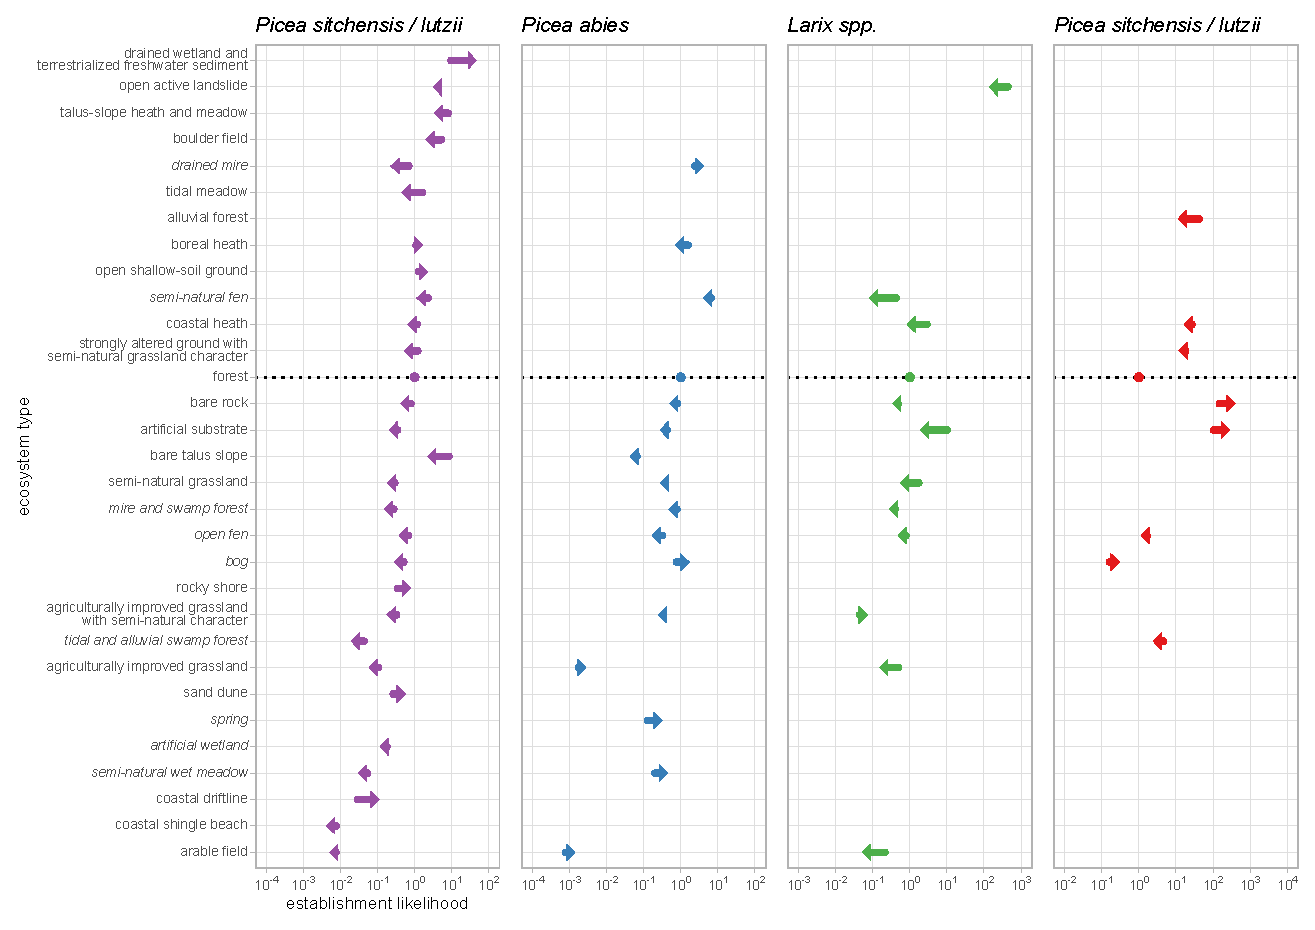
\includegraphics{/home/julien/Documents/dissertation/chapter3/conifer-plantation-spread/ms/figures/establishment-sensitivity.pdf}
\caption{\label{fig:establishment-sensitivity}Shifts in estimated relative establishment likelihoods when relative seed rain (from the WALD dispersal model) is included in the model as a covariate rather than an offset. Arrows point from the models with with offsets to the models with covariates.}
\end{figure}

\end{landscape}
\newpage

\hypertarget{references}{%
\section*{References}\label{references}}
\addcontentsline{toc}{section}{References}

\hypertarget{refs}{}
\leavevmode\hypertarget{ref-albertLanduseChangeSubalpine2008}{}%
Albert, C. H., Thuiller, W., Lavorel, S., Davies, I. D., \& Garbolino, E. (2008). Land-use change and subalpine tree dynamics: Colonization of Larix decidua in French subalpine grasslands. \emph{Journal of Applied Ecology}, \emph{45}(2), 659--669. \url{https://doi.org/10.1111/j.1365-2664.2007.01416.x}

\leavevmode\hypertarget{ref-appelgrenKartleggingAvKortdistansespredning2018}{}%
Appelgren, L. (2018). \emph{Kartlegging av kortdistansespredning av fremmede bartrær i Rogaland 2018} (Nos. 644). Ecofact.

\leavevmode\hypertarget{ref-appelgrenKartleggingAvKortdistansespredning2017}{}%
Appelgren, L., \& Torvik, S. E. (2017). \emph{Kartlegging av kortdistansespredning av fremmede bartrær i Rogaland og Hordaland} (Nos. 607). Ecofact.

\leavevmode\hypertarget{ref-bakkestuenSteplessModelsRegional2008}{}%
Bakkestuen, V., Erikstad, L., \& Halvorsen, R. (2008). Step-less models for regional environmental variation in Norway. \emph{Journal of Biogeography}, \emph{35}(10), 1906--1922. \url{https://doi.org/10.1111/j.1365-2699.2008.01941.x}

\leavevmode\hypertarget{ref-bianchiMethodsPredictingSitka2019}{}%
Bianchi, S., Hale, S., \& Gibbons, J. (2019). Methods for predicting Sitka spruce natural regeneration presence and density in the UK. \emph{iForest - Biogeosciences and Forestry}, \emph{12}(3), 279. \url{https://doi.org/10.3832/ifor2888-012}

\leavevmode\hypertarget{ref-blasco-morenoWhatDoesZero2019}{}%
Blasco-Moreno, A., Pérez-Casany, M., Puig, P., Morante, M., \& Castells, E. (2019). What does a zero mean? Understanding false, random and structural zeros in ecology. \emph{Methods in Ecology and Evolution}, \emph{10}(7), 949--959. \url{https://doi.org/10.1111/2041-210X.13185}

\leavevmode\hypertarget{ref-brooksStatisticalModelingPatterns2019}{}%
Brooks, M. E., Kristensen, K., Darrigo, M. R., Rubim, P., Uriarte, M., Bruna, E., \& Bolker, B. M. (2019). Statistical modeling of patterns in annual reproductive rates. \emph{Ecology}, \emph{100}(7), e02706. \url{https://doi.org/10.1002/ecy.2706}

\leavevmode\hypertarget{ref-brooksGlmmTMBBalancesSpeed2017}{}%
Brooks, M. E., Kristensen, K., van Benthem, K. J., Magnusson, A., Berg, C. W., Nielsen, A., Skaug, H. J., Maechler, M., \& Bolker, B. M. (2017). glmmTMB balances speed and flexibility among packages for zero-inflated generalized linear mixed modeling. \emph{The R Journal}, \emph{9}(2), 378--400.

\leavevmode\hypertarget{ref-brunduGlobalGuidelinesSustainable2020}{}%
Brundu, G., Pauchard, A., Pyšek, P., Pergl, J., Bindewald, A. M., Brunori, A., Canavan, S., Campagnaro, T., Celesti-Grapow, L., de Sá Dechoum, M., Dufour-Dror, J.-M., Essl, F., Flory, S. L., Genovesi, P., Guarino, F., Guangzhe, L., Hulme, P. E., Jager, H., Kettle, C. J., \ldots{} Richardson, D. M. (2020). Global guidelines for the sustainable use of non-native trees to prevent tree invasions and mitigate their negative impacts. \emph{Neobiota}, \emph{61}, 65--116. \url{https://doi.org/10.3897/neobiota.65.58380}

\leavevmode\hypertarget{ref-brynVeilederKartleggingAv2015}{}%
Bryn, A., \& Halvorsen, R. (2015). \emph{Veileder for kartlegging av terrestrisk naturvariasjon etter NiN 2.0. Veileder versjon 2.0.0.} Norwegian Biodiversity Information Facility.

\leavevmode\hypertarget{ref-bullockAllDispersalFunctions2018}{}%
Bullock, J. M., Hooftman, D. A. P., Tamme, R., Götzenberger, L., Pärtel, M., González, L. M., \& White, S. M. (2018). All dispersal functions are wrong, but many are useful: A response to Cousens et al. \emph{Journal of Ecology}, \emph{106}(3), 907--910. \url{https://doi.org/10.1111/1365-2745.12890}

\leavevmode\hypertarget{ref-bullockSynthesisEmpiricalPlant2017}{}%
Bullock, J. M., Mallada González, L., Tamme, R., Götzenberger, L., White, S. M., Pärtel, M., Hooftman, D. A. P., \& Rees, M. (2017). A synthesis of empirical plant dispersal kernels. \emph{Journal of Ecology}, \emph{105}(1), 6--19. \url{https://doi.org/10.1111/1365-2745.12666}

\leavevmode\hypertarget{ref-catfordQuantifyingLevelsBiological2012}{}%
Catford, J. A., Vesk, P. A., Richardson, D. M., \& Pyšek, P. (2012). Quantifying levels of biological invasion: Towards the objective classification of invaded and invasible ecosystems. \emph{Global Change Biology}, \emph{18}(1), 44--62. \url{https://doi.org/10.1111/j.1365-2486.2011.02549.x}

\leavevmode\hypertarget{ref-chytrySeparatingHabitatInvasibility2008}{}%
Chytrý, M., Jarošík, V., Pyšek, P., Hájek, O., Knollová, I., Tichý, L., \& Danihelka, J. (2008). Separating Habitat Invasibility by Alien Plants from the Actual Level of Invasion. \emph{Ecology}, \emph{89}(6), 1541--1553. \url{https://doi.org/10.1890/07-0682.1}

\leavevmode\hypertarget{ref-chytryHabitatInvasionsAlien2008}{}%
Chytrý, M., Maskell, L. C., Pino, J., Pyšek, P., Vilà, M., Font, X., \& Smart, S. M. (2008). Habitat invasions by alien plants: A quantitative comparison among Mediterranean, subcontinental and oceanic regions of Europe. \emph{Journal of Applied Ecology}, \emph{45}(2), 448--458. \url{https://doi.org/10.1111/j.1365-2664.2007.01398.x}

\leavevmode\hypertarget{ref-despainDispersalEcologyLodgepole2001}{}%
Despain, D. G. (2001). Dispersal ecology of lodgepole pine (Pinus contorta Dougl.) In its native environment as related to Swedish forestry. \emph{Forest Ecology and Management}, \emph{141}(1), 59--68. \url{https://doi.org/10.1016/S0378-1127(00)00489-8}

\leavevmode\hypertarget{ref-dovciakSeedRainEnvironmental2008}{}%
Dovčiak, M., Hrivnák, R., Ujházy, K., \& Gömöry, D. (2008). Seed rain and environmental controls on invasion of Picea abies into grassland. \emph{Plant Ecology}, \emph{194}(1), 135--148. \url{https://doi.org/10.1007/s11258-007-9280-2}

\leavevmode\hypertarget{ref-fernandesWhatDrivesEucalyptus2018}{}%
Fernandes, P., Máguas, C., Correia, O., \& González-Moreno, P. (2018). What drives Eucalyptus globulus natural establishment outside plantations? The relative importance of climate, plantation and site characteristics. \emph{Biological Invasions}, \emph{20}(5), 1129--1146. \url{https://doi.org/10.1007/s10530-017-1614-y}

\leavevmode\hypertarget{ref-haakenstadNORA10EIRevisedRegional2020}{}%
Haakenstad, H., Breivik, Ø., Reistad, M., \& Aarnes, O. J. (2020). NORA10EI: A revised regional atmosphere-wave hindcast for the North Sea, the Norwegian Sea and the Barents Sea. \emph{International Journal of Climatology}, \emph{40}(10), 4347--4373. \url{https://doi.org/10.1002/joc.6458}

\leavevmode\hypertarget{ref-haakenstad15yearHighResolution2017}{}%
Haakenstad, H., \& Haugen, J. E. (2017). \emph{A 15-year high resolution meteorological dataset for risk assessment in southern Norway} (METreport 5/2017). Norwegian Meteorological Institute.

\leavevmode\hypertarget{ref-halvorsenNaturNorgeNiN2015}{}%
Halvorsen, R., Bryn, A., Erikstad, L., \& Lindgaard, A. (2015). \emph{Natur i Norge (NiN). Versjon 2.0.0.} (pp. 1--26). Norwegian Biodiversity Information Facility.

\leavevmode\hypertarget{ref-halvorsenSystematicsEcodiversityEcoSyst2020}{}%
Halvorsen, R., Skarpaas, O., Bryn, A., Bratli, H., Erikstad, L., Simensen, T., \& Lieungh, E. (2020). Towards a systematics of ecodiversity: The EcoSyst framework. \emph{Global Ecology and Biogeography}, \emph{29}(11), 1887--1906. \url{https://doi.org/10.1111/geb.13164}

\leavevmode\hypertarget{ref-hartigDHARMaResidualDiagnostics2020}{}%
Hartig, F. (2020). \emph{DHARMa: Residual diagnostics for hierarchical (multi-level / mixed) regression models} {[}Manual{]}.

\leavevmode\hypertarget{ref-kargerClimatologiesHighResolution2017}{}%
Karger, D. N., Conrad, O., Böhner, J., Kawohl, T., Kreft, H., Soria-Auza, R. W., Zimmermann, N. E., Linder, H. P., \& Kessler, M. (2017). Climatologies at high resolution for the earth's land surface areas. \emph{Scientific Data}, \emph{4}, 170122. \url{https://doi.org/10.1038/sdata.2017.122}

\leavevmode\hypertarget{ref-katulMechanisticAnalyticalModels2005}{}%
Katul, G., Porporato, A., Nathan, R., Siqueira, M., Soons, M., Poggi, D., Horn, H., \& Levin, S. (2005). Mechanistic analytical models for long-distance seed dispersal by wind. \emph{The American Naturalist}, \emph{166}(3), 368--381.

\leavevmode\hypertarget{ref-kyrkjeeideKartleggingAvKortdistansespredning2017}{}%
Kyrkjeeide, M. O., Often, A., Myklebost, H. E., Olsen, S. L., Hagelin, J., Ruano, M., Frivoll, V., \& De Stefano, M. (2017). \emph{Kartlegging av kortdistansespredning av fremmede bartrær Nord Norge} (Nos. 1427). NINA.

\leavevmode\hypertarget{ref-langdonPinusContortaInvasion2010}{}%
Langdon, B., Pauchard, A., \& Aguayo, M. (2010). Pinus contorta invasion in the Chilean Patagonia: Local patterns in a global context. \emph{Biological Invasions}, \emph{12}(12), 3961--3971. \url{https://doi.org/10.1007/s10530-010-9817-5}

\leavevmode\hypertarget{ref-macekLifeDeathPicea2017}{}%
Macek, M., Wild, J., Kopecký, M., Červenka, J., Svoboda, M., Zenáhlíková, J., Brůna, J., Mosandl, R., \& Fischer, A. (2017). Life and death of Picea abies after bark-beetle outbreak: Ecological processes driving seedling recruitment. \emph{Ecological Applications}, \emph{27}(1), 156--167. \url{https://doi.org/10.1002/eap.1429}

\leavevmode\hypertarget{ref-mcconnachieEstimatingEffectPlantations2015}{}%
McConnachie, M. M., Wilgen, B. W. van, Richardson, D. M., Ferraro, P. J., \& Forsyth, A. T. (2015). Estimating the effect of plantations on pine invasions in protected areas: A case study from South Africa. \emph{Journal of Applied Ecology}, \emph{52}(1), 110--118. \url{https://doi.org/10.1111/1365-2664.12366}

\leavevmode\hypertarget{ref-mcelreathHauntedDAGCausal2020}{}%
McElreath, R. (2020). The Haunted DAG \& The Causal Terror. In \emph{Statisitical Rethinking: A Bayesian Course with Examples in R and Stan} (Second).

\leavevmode\hypertarget{ref-millerHowDisturbanceHistory2021}{}%
Miller, A. D., Inamine, H., Buckling, A., Roxburgh, S. H., \& Shea, K. (2021). How disturbance history alters invasion success: Biotic legacies and regime change. \emph{Ecology Letters}, \emph{n/a}(n/a). \url{https://doi.org/10.1111/ele.13685}

\leavevmode\hypertarget{ref-nygaardSpreadIntroducedSitka2017}{}%
Nygaard, P., \& Øyen, B.-H. (2017). Spread of the introduced Sitka spruce (Picea sitchensis) in coastal Norway. \emph{Forests}, \emph{8}(1), 24. \url{https://doi.org/10.3390/f8010024}

\leavevmode\hypertarget{ref-olsenKartleggingAvKortdistansespredning2019}{}%
Olsen, S. L., Kyrkjeeide, M. O., Myklebost, H. E., Jackson, C., \& Gastinger, M.-M. (2019). \emph{Kartlegging av kortdistansespredning av fremmede bartrær} (Nos. 1728). NINA.

\leavevmode\hypertarget{ref-olsenKartleggingAvKortdistansespredning2016}{}%
Olsen, S. L., Stabbetorp, O., Skarpaas, O., Often, A., \& Gajda, H. (2016). \emph{Kartlegging av kortdistansespredning av fremmede bartrær Vrifuru (Pinus contorta) og lutzgran (Picea lutzii)} (Nos. 1231). NINA.

\leavevmode\hypertarget{ref-petersonEcologyManagementSitka1997}{}%
Peterson, E. B., Peterson, N. M., Weetman, G. F., \& Martin, P. J. (1997). \emph{Ecology and management of Sitka spruce, emphasizing its natural range in British Colombia}. UBC Press.

\leavevmode\hypertarget{ref-pysekScientistsWarningInvasive2020}{}%
Pyšek, P., Hulme, P. E., Simberloff, D., Bacher, S., Blackburn, T. M., Carlton, J. T., Dawson, W., Essl, F., Foxcroft, L. C., Genovesi, P., Jeschke, J. M., Kühn, I., Liebhold, A. M., Mandrak, N. E., Meyerson, L. A., Pauchard, A., Pergl, J., Roy, H. E., Seebens, H., \ldots{} Richardson, D. M. (2020). Scientists' warning on invasive alien species. \emph{Biological Reviews}, \emph{95}(6), 1511--1534. \url{https://doi.org/10.1111/brv.12627}

\leavevmode\hypertarget{ref-rcoreteamLanguageEnvironmentStatistical2020}{}%
R Core Team. (2020). \emph{R: A language and environment for statistical computing}. R Foundation for Statistical Computing.

\leavevmode\hypertarget{ref-reistadHighresolutionHindcastWind2011}{}%
Reistad, M., Breivik, Ø., Haakenstad, H., Aarnes, O. J., Furevik, B. R., \& Bidlot, J.-R. (2011). A high-resolution hindcast of wind and waves for the North Sea, the Norwegian Sea, and the Barents Sea. \emph{Journal of Geophysical Research: Oceans}, \emph{116}, C05019. \url{https://doi.org/10.1029/2010JC006402}

\leavevmode\hypertarget{ref-richardsonNaturalizationIntroducedPlants2012}{}%
Richardson, D. M., \& Pyšek, P. (2012). Naturalization of introduced plants: Ecological drivers of biogeographical patterns. \emph{New Phytologist}, \emph{196}(2), 383--396. \url{https://doi.org/10.1111/j.1469-8137.2012.04292.x}

\leavevmode\hypertarget{ref-richardsonConifersInvasiveAliens2004}{}%
Richardson, D. M., \& Rejmánek, M. (2004). Conifers as invasive aliens: A global survey and predictive framework. \emph{Diversity and Distributions}, \emph{10}, 321--331.

\leavevmode\hypertarget{ref-rougetInferringProcessPattern2003}{}%
Rouget, M., \& Richardson, D. M. (2003). Inferring Process from Pattern in Plant Invasions: A Semimechanistic Model Incorporating Propagule Pressure and Environmental Factors. \emph{The American Naturalist}, \emph{162}(6), 713--724. \url{https://doi.org/10.1086/379204}

\leavevmode\hypertarget{ref-sandvenKartleggingAvKortdistansespredning2019}{}%
Sandven, J., Aamodt, O. W., \& Sørhuus, Ø. (2019). \emph{Kartlegging av kortdistansespredning av fremmede bartrær i Hordaland} (6/2019). NORSKOG.

\leavevmode\hypertarget{ref-skarpaasDispersalPatternsDispersal2007}{}%
Skarpaas, O., \& Shea, K. (2007). Dispersal Patterns, Dispersal Mechanisms, and Invasion Wave Speeds for Invasive Thistles. \emph{The American Naturalist}, \emph{170}(3), 421--430. \url{https://doi.org/10.1086/519854}

\leavevmode\hypertarget{ref-taylorDriversPlantInvasion2016}{}%
Taylor, K. T., Maxwell, B. D., Pauchard, A., Nuñez, M. A., Peltzer, D. A., Terwei, A., \& Rew, L. J. (2016). Drivers of plant invasion vary globally: Evidence from pine invasions within six ecoregions. \emph{Global Ecology and Biogeography}, \emph{25}(1), 96--106. \url{https://doi.org/10.1111/geb.12391}

\leavevmode\hypertarget{ref-textorRobustCausalInference2016}{}%
Textor, J., van der Zander, B., Gilthorpe, M. S., Liśkiewicz, M., \& Ellison, G. T. (2016). Robust causal inference using directed acyclic graphs: The R package ``dagitty''. \emph{International Journal of Epidemiology}, \emph{45}(6), 1887--1894. \url{https://doi.org/10.1093/ije/dyw341}

\leavevmode\hypertarget{ref-tingstadTemperaturePrecipitationBiotic2015}{}%
Tingstad, L., Olsen, S. L., Klanderud, K., Vandvik, V., \& Ohlson, M. (2015). Temperature, precipitation and biotic interactions as determinants of tree seedling recruitment across the tree line ecotone. \emph{Oecologia}, \emph{179}(2), 599--608. \url{https://doi.org/10.1007/s00442-015-3360-0}

\leavevmode\hypertarget{ref-vikaneInvasionCallunaHeath2013}{}%
Vikane, J. H., Vandvik, V., \& Vetaas, O. R. (2013). Invasion of Calluna heath by native and non-native conifers: The role of succession, disturbance and allelopathy. \emph{Plant Ecology}, \emph{214}(7), 975--985. \url{https://doi.org/10.1007/s11258-013-0223-9}

\leavevmode\hypertarget{ref-westreichTableFallacyPresenting2013}{}%
Westreich, D., \& Greenland, S. (2013). The Table 2 Fallacy: Presenting and Interpreting Confounder and Modifier Coefficients. \emph{American Journal of Epidemiology}, \emph{177}(4), 292--298. \url{https://doi.org/10.1093/aje/kws412}

\leavevmode\hypertarget{ref-zuurMixedEffectsModels2009}{}%
Zuur, A. F., Ieno, E. N., Walker, N., Saveliev, A. A., \& Smith, G. M. (2009). \emph{Mixed effects models and extensions in ecology with R} (M. Gail, K. Krickeberg, J. Samet, A. Tsiatis, \& W. Wong, Eds.). Springer New York. \url{https://doi.org/10.1007/978-0-387-87458-6}

\end{document}
